\chapter[Computer Graphics Primer]{Computer\\ Graphics\\ Primer}
\label{chap:computer_graphics_primer}

% Position the image to the right of the heading.
\vspace{-11\baselineskip} % move up
\hfill
 \begin{minipage}{0.5\textwidth}
 \centering
 %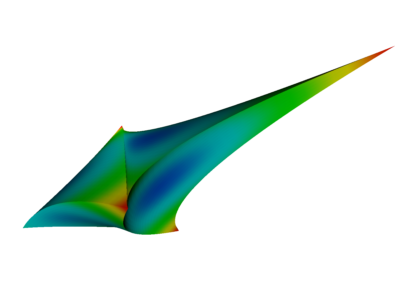
\includegraphics[width=0.98\linewidth]{VTKTextbook-12}
 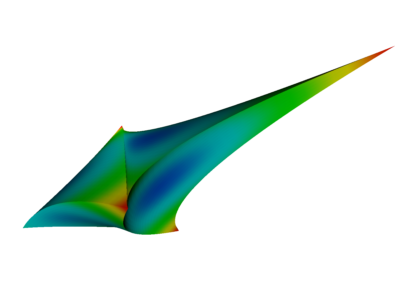
\includegraphics{VTKTextbook-12}
  \captionof*{figure}{\textit{Rendering quadratic tetrahedra.}}
 \end{minipage}
\vspace{2\baselineskip}


\firstletter{C}omputer graphics is the foundation of data visualization. Practically speaking, visualization is the process that transforms data into a set of graphics primitives. The methods of computer graphics are then used to convert these primitives into pictures or animations. This chapter discusses basic computer graphics principles. We begin by describing how lights and physical objects interact to form what we see. Next we examine how to simulate these interactions using computer graphics techniques. Hardware issues play an important role here since modern computers have built-in hardware support for graphics. The chapter concludes with a series of examples that illustrate our object--oriented model for 3D computer graphics.

\section{Introduction}

Computer graphics\index{computer graphics} is the process of generating images using computers. We call this process \emph{rendering}\index{rendering|(}. There are many types of rendering processes, ranging from 2D paint programs to sophisticated 3D techniques. In this chapter we focus on basic 3D techniques for visualization.

We can view rendering as the process of converting graphical data into an image. In data visualization our goal is to transform data into graphical data, or \emph{graphics primitives}, that are then rendered. The goal of our rendering is not so much photo realism as it is information content. We also strive for interactive graphical displays with which it is possible to directly manipulate the underlying data. This chapter explains the process of rendering an image from graphical data. We begin by looking at the way lights, cameras, and objects (or actors) interact in the world around us. From this foundation we explain how to simulate this process on a computer.

\section{A Physical Description of Rendering}

\begin{figure}[ht]
  \centering
  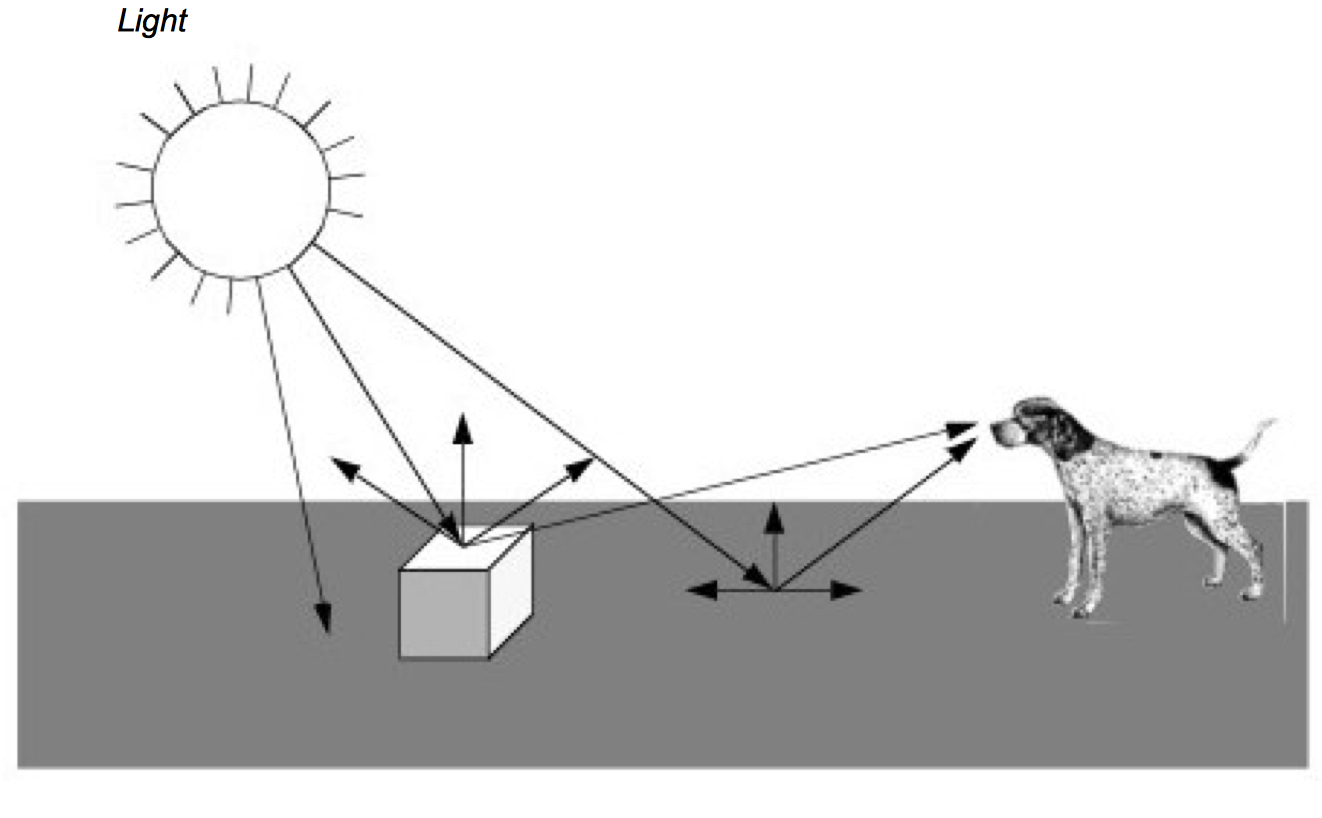
\includegraphics[width=0.8\textwidth]{Figure3-1}\\
  \caption{Physical generation of an image.}\label{fig:Figure3-1}
\end{figure}

Figure \ref{fig:Figure3-1} presents a simplified view of what happens when we look at an object, in this case a cube. Rays of light are emitted from a light source in all directions. (In this example we assume that the light source is the sun.) Some of these rays happen to strike the cube whose surface absorbs some of the incident light and reflects the rest of it. Some of this reflected light may head towards us and enter our eyes. If this happens, then we ``see'' the object. Likewise, some of the light from the sun will strike the ground and some small percentage of it will be reflected into our eyes.

As you can imagine, the chances of a ray of light traveling from the sun through space to hit a small object on a relatively small planet are low. This is compounded by the slim odds that the ray of light will reflect off the object and into our eyes. The only reason we can see is that the sun produces such an enormous amount of light that it overwhelms the odds. While this may work in real life, trying to simulate it with a computer can be difficult. Fortunately, there are other ways to look at this problem.

A common and effective technique for 3D computer graphics is called \emph{ray--tracing}\index{ray--tracing} or \emph{ray--casting}. Ray--tracing simulates the interaction of light with objects by following the path of each light ray. Typically, we follow the ray backwards from the viewer's eyes and into the world to determine what the ray strikes. The direction of the ray is in the direction we are looking (i.e., the view direction) including effects of perspective (if desired). When a ray intersects an object, we can determine if that point is being lit by our light source. This is done by tracing a ray from the point of intersection towards the light. If the ray intersects the light, then the point is being lit. If the ray intersects something else before it gets to the light, then that light will not contribute to illuminating the point. For multiple light sources we just repeat this process for each light source. The total contributions from all the light sources, plus any ambient scattered light, will determine the total lighting or shadow for that point. By following the light's path backwards, ray tracing only looks at rays that end up entering the viewer's eyes. This dramatically reduces the number of rays that must be computed by a simulation program.

Having described ray tracing as a rendering process, it may be surprising that many members of the graphics community do not use it. This is because ray tracing is a relatively slow image generation method since it is typically implemented in software. Other graphics techniques have been developed that generate images using dedicated computer hardware. To understand why this situation has emerged, it is instructive to briefly examine the taxonomy and history of computer graphics.

\subsection{Image--Order and Object--Order Methods}

Rendering processes can be broken into two categories: \emph{image-order}\index{image--order rendering}\index{rendering!image--order} and \emph{object-order}\index{object--order rendering}\index{rendering!object--order}. Ray tracing is an image--order process. It works by determining what happens to each ray of light, one at a time. An object-order process works by rendering each object, one at a time. In the above example, an object-order technique would proceed by first rendering the ground and then the cube.

To look at it another way consider painting a picture of a barn. Using an image-order algorithm you would start at the upper left corner of the canvas and put down a drop of the correct color paint. (Each paint drop is called a picture element or \emph{pixel}\index{pixel}.) Then you would move a little to the right and put down another drop of paint. You would continue until you reached the right edge of the canvas, then you would move down a little and start on the next row. Each time you put down a drop of paint you make certain it is the correct color for each pixel on the canvas. When you are done you will have a painting of a barn.

An alternative approach is based on the more natural (at least for many people) object-order process. We work by painting the different objects in our scene, independent of where the objects actually are located on the scene. We may paint from back to front, front-to-back, or in arbitrary order. For example, we could start by painting the sky and then add in the ground. After these two objects were painted we would then add in the barn. In the image-order process we worked on the canvas in a very orderly fashion; left to right, top to bottom. With an object-order process we tend to jump from one part of the canvas to another, depending on what object we are drawing.

The field of computer graphics started out using object-order processes. Much of the early work was closely tied to the hardware display device, initially a vector display. This was little more than an oscilloscope, but it encouraged graphical data to be drawn as a series of line segments. As the original vector displays gave way to the currently ubiquitous raster displays, the notion of representing graphical data as a series of objects to be drawn was preserved. Much of the early work pioneered by Bresenham \cite{Bresenham65} at IBM focused on how to properly convert line segments into a form that would be suitable for line plotters. The same work was applied to the task of rendering lines onto the raster displays that replaced the oscilloscope. Since then the hardware has become more powerful and capable of displaying much more complex primitives than lines.

It wasn't until the early 1980s that a paper by Turner Whitted \cite{Whitted80} prompted many people to look at rendering from a more physical perspective. Eventually ray tracing became a serious competitor to the traditional object--order rendering techniques, due in part to the highly realistic images it can produce. Object--order rendering has maintained its popularity because there is a wealth of graphics hardware designed to quickly render objects. Ray tracing tends to be done without any specialized hardware and therefore is a time-consuming process.

\subsection{Surface versus Volume Rendering}

The discussion to this point in the text has tacitly assumed that when we render an object, we are viewing the surfaces of objects and their interactions with light. However, common objects such as clouds, water, and fog, are translucent, or scatter light that passes through them. Such objects cannot be rendered using a model based exclusively on surface interactions. Instead, we need to consider the changing properties inside the object to properly render them. We refer to these two rendering models as \emph{surface rendering} (i.e., render the surfaces of an object) and \emph{volume rendering}\index{volume rendering} (i.e., render the surface and interior of an object).

Generally speaking, when we render an object using surface rendering\index{rendering!surface}\index{surface rendering} techniques, we mathematically model the object with a surface description such as points, lines, triangles, polygons, or 2D and 3D splines. The interior of the object is not described, or only implicitly represented from the surface representation (i.e., surface is the boundary of the volume). Although techniques do exist that allow us to make the surface transparent or translucent, there are still many phenomena that cannot be simulated using surface rendering techniques alone (e.g., scattering or light emission). This is particularly true if we are trying to render data interior to an object, such as X-ray intensity from a CT scan.

Volume rendering\index{rendering!volume} techniques allow us to see the inhomogeneity inside objects. In the prior CT example, we can realistically reproduce X-ray images by considering the intensity values from both the surface and interior of the data. Although it is premature to describe this process at this point in the text, you can imagine extending our ray tracing example from the previous section. Thus rays not only interact with the surface of an object, they also interact with the interior.

In this chapter we focus on surface rendering techniques. While not as powerful as volume rendering, surface rendering is widely used because it is relatively fast compared to volumetric techniques, and allows us to create images for a wide variety of data and objects. Chapter 7: \nameref{chap:advanced_computer_graphics} describes volume rendering in more detail.
\index{rendering|)}

\subsection{Visualization Not Graphics}

Although the authors would enjoy providing a thorough treatise on computer graphics, such a discourse is beyond the scope of this text. Instead we make the distinction between visualization (exploring, transforming, and mapping data) and computer graphics (mapping and rendering). The focus will be on the principles and practice of visualization, and not on 3D computer graphics. In this chapter and Chapter 7: \nameref{chap:advanced_computer_graphics} we introduce basic concepts and provide a working knowledge of 3D computer graphics. For those more interested in this field, we refer you to the texts recommended in the ``Bibliographic Notes'' on page \pageref{Ch03BibNotes} at the end of this chapter.

One of the regrets we have regarding this posture is that certain rendering techniques are essentially visualization techniques. We see this hinted at in the previous paragraph, where we use the term "mapping" to describe both visualization and computer graphics. There is not currently and will likely never be a firm distinction between visualization and graphics. For example, many researchers consider volume rendering to be squarely in the field of visualization because it addresses one of the most important forms of visualization data. Our distinction is mostly for our own convenience, and offers us the opportunity to finish this text. We recommend that a serious student of visualization supplement the material presented here with deeper books on computer graphics and volume rendering.

In the next few pages we describe the rendering process in more detail. We start by describing several color models. Next we examine the primary components of the rendering process. There are sources of light such as the sun, objects we wish to render such as a cube or sphere (we refer to these objects as actors), and there is a camera that looks out into the world. These terms are taken from the movie industry and tend to be familiar to most people. Actors\index{actor} represent graphical data or objects, lights illuminate the actors, and the camera constructs a picture by projecting the actors onto a view plane. We call the combination of lights, camera, and actors the scene, and refer to the rendering process as rendering the scene.

\section{Color}
\label{sec:color}
\index{color|(}

The electromagnetic spectrum visible to humans contains wavelengths ranging from about 400 to 700 nanometers. The light that enters our eyes consists of different \emph{intensities}\index{intensity} of these wavelengths, an example of which is shown in Figure \ref{fig:Figure3-2}. This intensity plot defines the color of the light, therefore a different plot results in a different color. Unfortunately, we may not notice the difference since the human eye throws out most of this information. There are three types of color receptors in the human eye called \emph{cones}. Each type responds to a subset of the 400 to 700 nanometer wave-length range as shown in Figure \ref{fig:Figure3-3}. Any color we see is encoded by our eyes into these three overlapping responses. This is a great reduction from the amount of information that actually comes into our eyes. As a result, the human eye is incapable of recognizing differences in any colors whose intensity curves, when applied to the human eye's response curves, result in the same triplet of responses. This also implies that we can store and represent colors in a computer using a simplified form without the human eye being able to recognize the difference.

\begin{figure}[!htb]
  \centering
  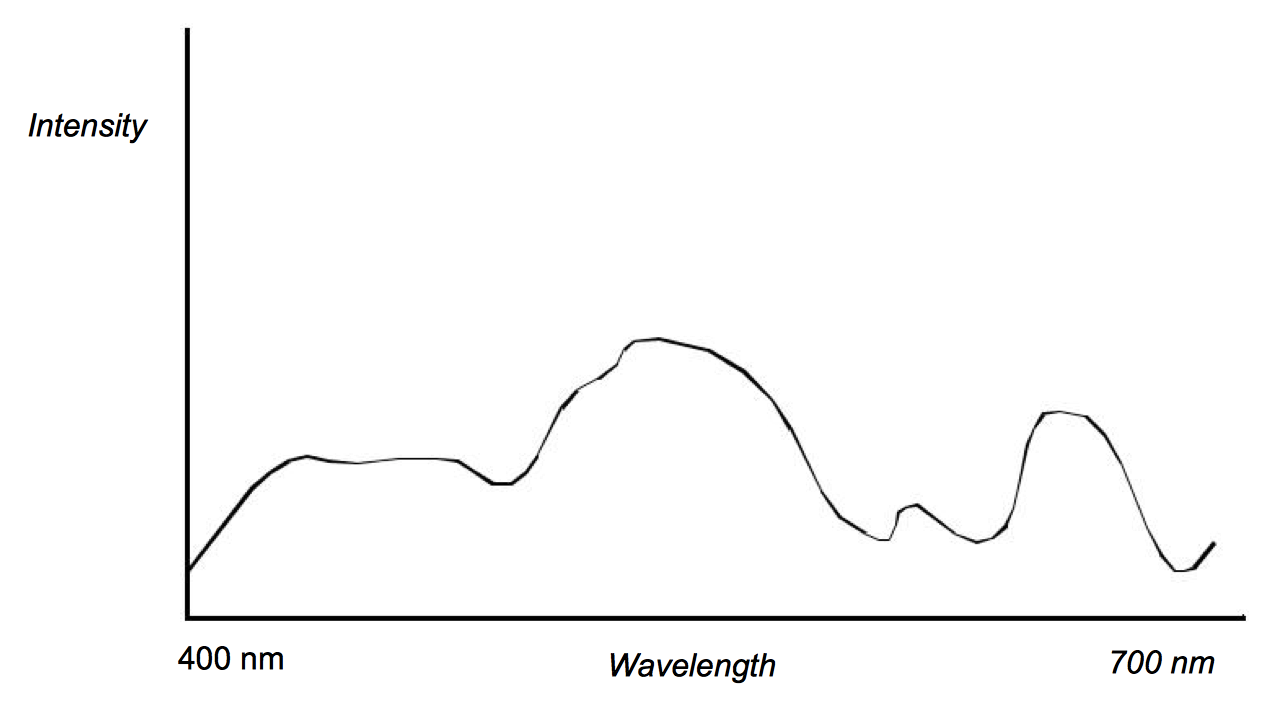
\includegraphics[width=0.8\textwidth]{Figure3-2}\\
  \caption{Wavelength versus Intensity plot.}\label{fig:Figure3-2}
\end{figure}

The two simplified component systems that we use to describe colors are RGB and HSV color systems. The RGB\index{RGB} system represents colors based on their red, green, and blue intensities. This can be thought of as a three dimensional space with the axes being red, green, and blue. Some common colors and their RGB components are shown in Table \ref{table:Figure3-4}.

The HSV\index{HSV} system represents colors based on their hue, saturation, and value. The value component is also known as the brightness or intensity component, and represents how much light is in the color. A value of 0.0 will always give you black and a value of 1.0 will give you something bright. The hue represents the dominant wavelength of the color and is often illustrated using a circle as in Figure \ref{fig:Figure3-5}. Each location on the circumference of this circle represents a different hue and can be specified using an angle. When we specify a hue we use the range from zero to one, where zero corresponds to zero degrees on the hue circle and one corresponds to 360 degrees. The saturation indicates how much of the hue is mixed into the color. For example, we can set the value to one, which gives us a bright color, and the hue to 0.66, to give us a dominant wavelength of blue. Now if we set the saturation to one, the color will be a bright primary blue. If we set the saturation to 0.5, the color will be sky blue, a blue with more white mixed in. If we set the saturation to zero, this indicates that there is no more of the dominant wavelength (hue) in the color than any other wavelength. As a result, the final color will be white (regardless of hue value). Table \ref{table:Figure3-4} lists HSV values for some common colors.

\begin{figure}[!htb]
  \centering
  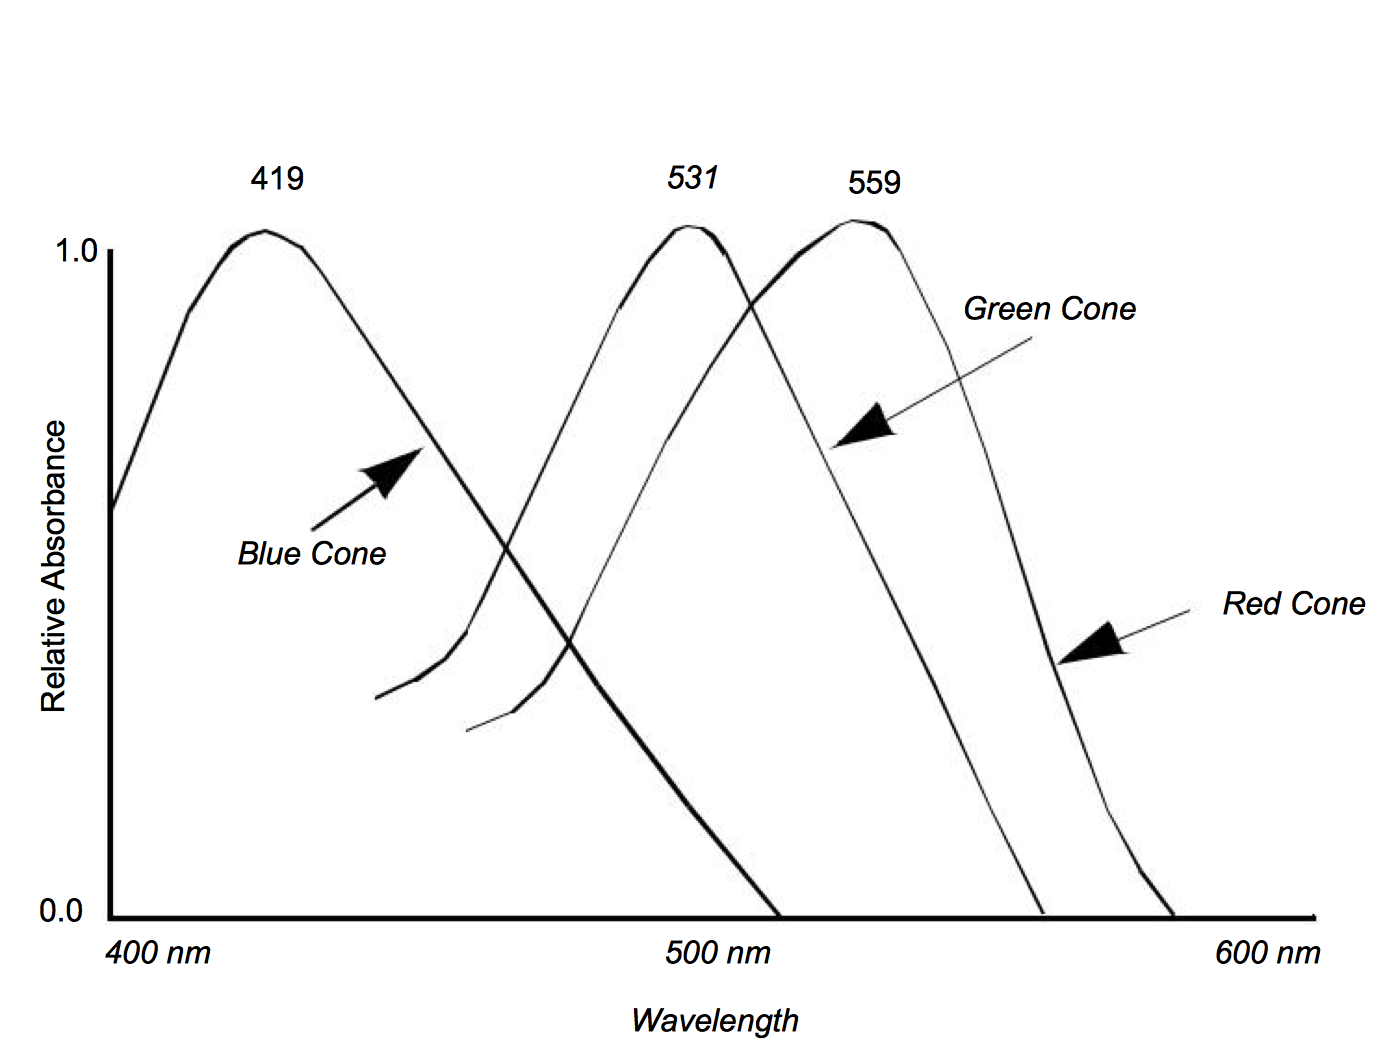
\includegraphics[width=0.8\textwidth]{Figure3-3}\\
  \caption{Relative absorbance of light by the three types of cones in the human retina.}\label{fig:Figure3-3}
\end{figure}

\begin{table}
	\centering
    \begin{tabular}{ | l | c | c | }
    \hline
    Color & RGB & HSV\\
    \hline
    Black & $0,0,0$ & $\ast,\ast,0$\\
    White & $1,1,1$ & $\ast,0,1$\\
    Red & $1,0,0$ & $0,1,1$\\
    Green & $0,1,0$ & $1/3,1,1$\\
    Blue & $0,0,1$ & $2/3,1,1$\\
    Cyan & $0,1,1$ & $1/2,1,1$\\
    Magenta & $1,0,1$ & $5/6,1,1$\\
    Yellow & $1,1,0$ & $1/6,1,1$\\
    Sky Blue & $1/2,1/2,1$ & $2/3,1/2,1$\\
    \hline
    \end{tabular}
    \caption{Common colors in RGB and HSV space}\label{table:Figure3-4}
\end{table}
  
\begin{figure}[!htb]
  \centering
  \begin{subfigure}[a]{0.6\textwidth}{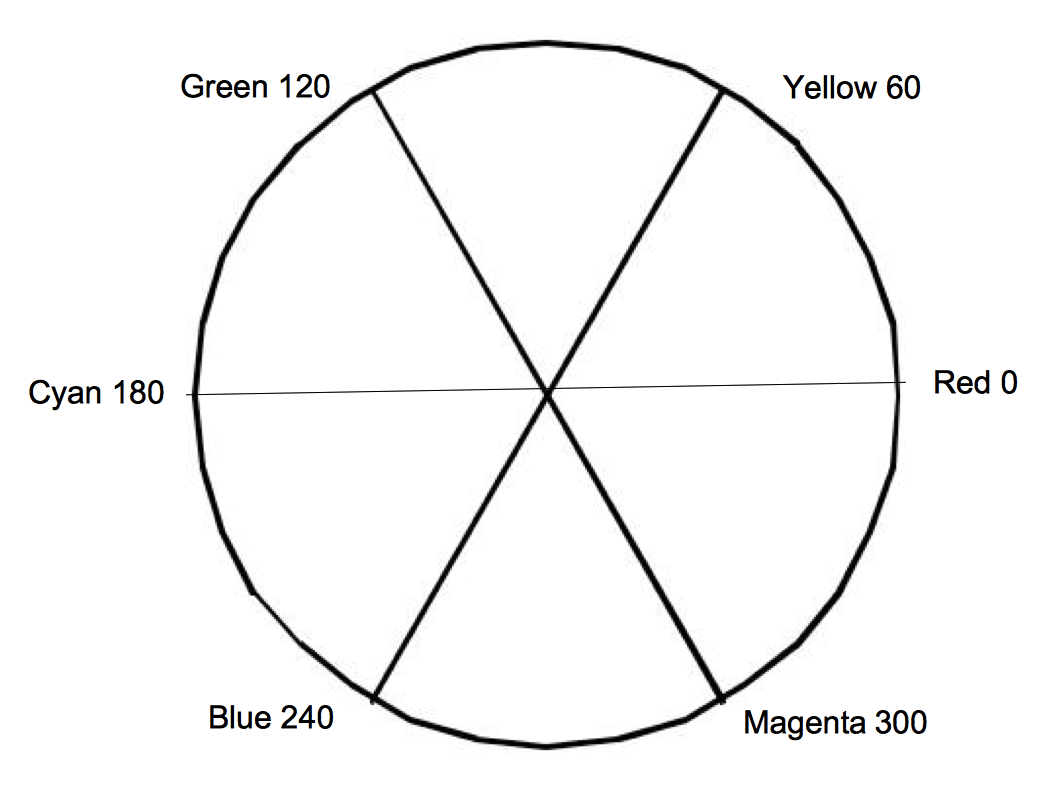
\includegraphics[width=\textwidth]{Figure3-5a}		  \label{fig:Figure3-5a}}
  \end{subfigure}
  \hfill
  \begin{subfigure}[b]{0.6\textwidth}{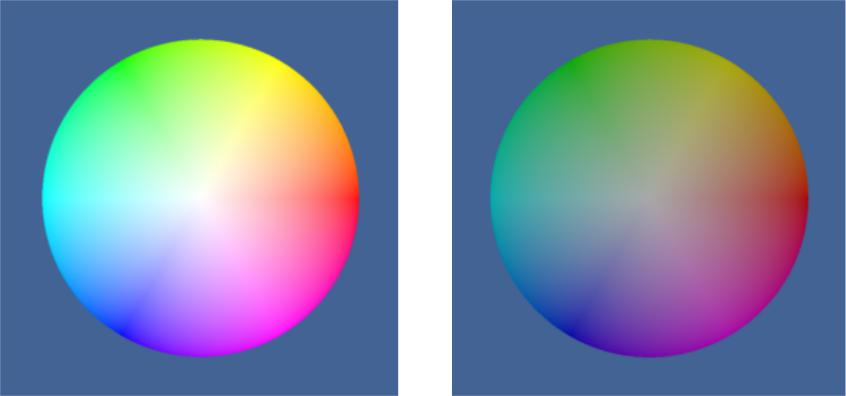
\includegraphics[width=\textwidth]{Figure3-5b}  	  \label{fig:Figure3-5b}}
  \end{subfigure}
  \caption{On the top, circular representation of hue. The other two
images on the bottom are slices through the HSV color space. The first slice
has a value of 1.0, the other has a value of 0.5.}
\label{fig:Figure3-5}
\end{figure}
\index{color|)}

\section{Lights}
\label{Lights}\index{light|(}

One of the major factors controlling the rendering process is the interaction of light with the actors in the scene. If there are no lights, the resulting image will be black and rather uninformative. To a great extent it is the interaction between the emitted light and the surface (and in some cases the interior) of the actors in the scene that defines what we see. Once rays of light interact with the actors in a scene, we have something for our camera to view.

Of the many different types of lights used in computer graphics, we will discuss the simplest, the infinitely distant, point light source. This is a simplified model compared to the lights we use at home and work. The light sources that we are accustomed to typically radiate from a region in space (a filament in an incandescent bulb, or a light-emitting gas in a fluorescent light). The point source lighting model assumes that the light is emitted in all directions from a single point in space. For an infinite light source, we assume that it is positioned infinitely far away from what it is illuminating. This is significant because it implies that the incoming rays from such a source will be parallel to each other. The emissions of a local light source, such as a lamp in a room, are not parallel. Figure \ref{fig:Figure3-6} illustrates the differences between a local light source with a finite volume, versus an infinite point light source. The intensity of the light emitted by our infinite light sources also remains constant as it travels, in contrast to the actual $1/distance^2$ relationship physical lights obey. As you can see this is a great simplification, which later will allow us to use less complex lighting equations.

\begin{figure}[!htb]
  \centering
  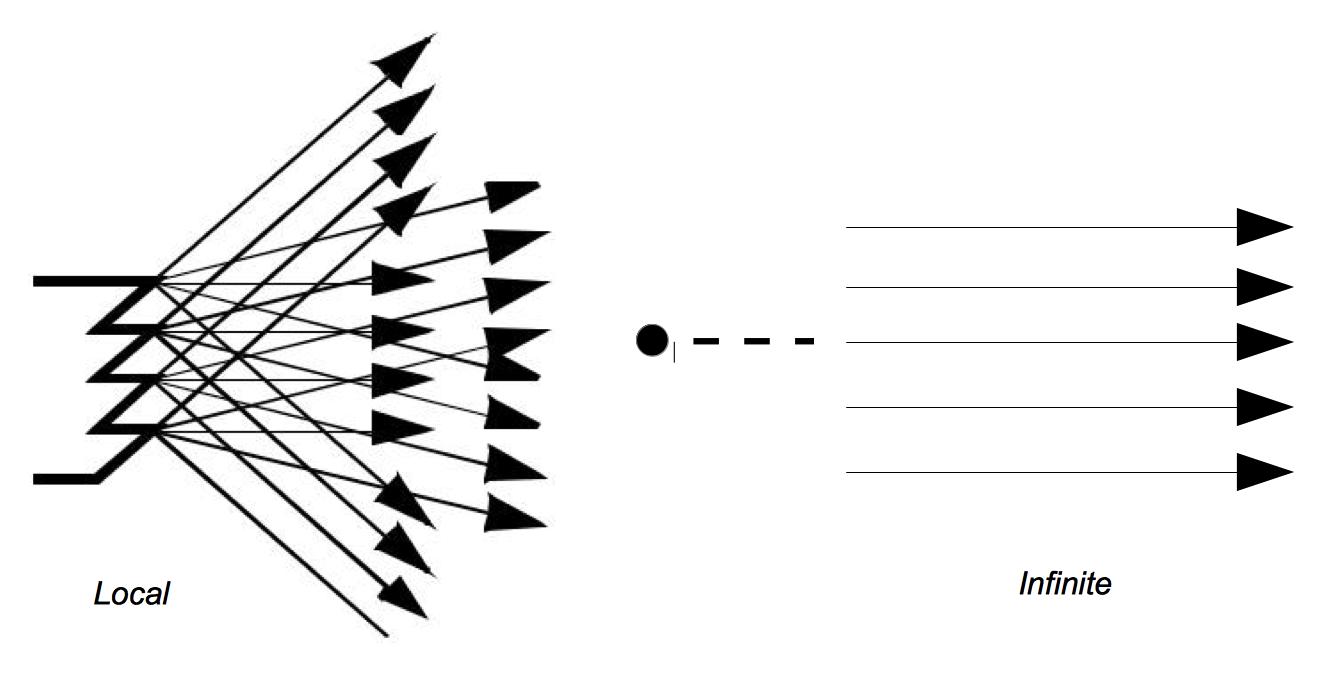
\includegraphics[width=0.8\textwidth]{Figure3-6}\\
  \caption{Local light source with a finite volume versus an infinite point light source.}\label{fig:Figure3-6}
\end{figure}

\section{Surface Properties}
\index{actor!surface properties|(}\index{surface properties|(}

As rays of light travel through space, some of them intersect our actors. When this happens, the rays of light interact with the surface of the actor to produce a color. Part of this resulting color is actually not due to direct light, but rather from \emph{ambient} light\index{ambient light}\index{light!ambient} that is being reflected or scattered from other objects. An ambient lighting model accounts for this and is a simple approximation of the complex scattering of light that occurs in the real world. It applies the intensity curve of the light source to the color of the object, also expressed as an intensity curve. The result is the color of the light we see when we look at that object. With such a model, it is important to realize that a white light shining on a blue ball is indistinguishable from a blue light shining on a white ball. The ambient lighting equation is

\begin{equation}\label{eq:3.1}
  R_a = L_c \cdot O_a
\end{equation}
\myequations{Ambient Lighting}

where $R_a$ is the resulting intensity curve due to ambient lighting, $L_c$ is the intensity curve of the ambient light, and $O_a$ is the color curve of the object. To help keep the equations simple we assume that all of the direction vectors are normalized (i.e., have a magnitude of one).

Two components of the resulting color depend on direct lighting. \emph{Diffuse lighting}\index{diffuse light}\index{light!diffuse}, which is also known as Lambertian reflection, takes into account the angle of incidence of the light onto an object. Figure \ref{fig:Figure3-7} shows the image of a cylinder that becomes darker as you move laterally from its center. The cylinder's color is constant; the amount of light hitting the surface of the cylinder changes. At the center, where the incoming light is nearly perpendicular to the surface of the cylinder, it receives more rays of light per surface area. As we move towards the side, this drops until finally the incoming light is parallel to the side of the cylinder and the resulting intensity is zero.

\begin{figure}[!htb]
  \centering
  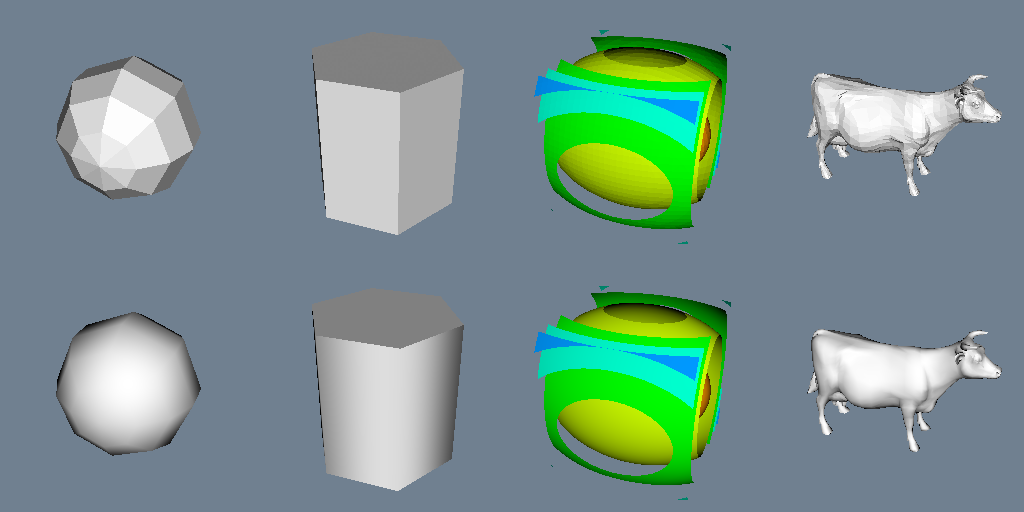
\includegraphics[width=0.8\textwidth]{Figure3-7}\\
  \caption{Flat and Gouraud shading. Different shading methods can dramatically improve the look of an object represented with polygons. On the top, flat shading uses a constant surface normal across each polygon. On the bottom, Gouraud shading interpolates normals from polygon vertices to give a smoother look.}\label{fig:Figure3-7}
\end{figure}

The contribution from diffuse lighting is expressed in Equation \ref{eq:3.2} and illustrated in Figure \ref{fig:Figure3-8}.

\begin{equation}\label{eq:3.2}
  R_d = L_cO_d[\overrightarrow{O}_n \cdot (-\overrightarrow{L}_n)]
\end{equation}
\myequations{Diffuse Lighting Contribution}

where $R_d$ is the resulting intensity curve due to diffuse lighting, $L_c$ is the intensity curve for the light, and $O_c$ is the color curve for the object. Notice that the diffuse light is a function of the relative angle between incident light vector and $\overrightarrow{L}_n$ and the surface normal of the object $\overrightarrow{O}_n$. As a result diffuse lighting is independent of viewer position.

\emph{Specular} lighting\index{specular light}\index{light!specular} represents direct reflections of a light source off a shiny object. Figure \ref{fig:Figure3-10} shows a diffusely lit ball with varying specular reflection. The specular intensity (which varies between the top and bottom rows) controls the intensity of the specular lighting. The specular power, $O_sp$, indicates how shiny an object is, more specifically it indicates how quickly specular reflections diminish as the reflection angles deviate from a perfect reflection. Higher values indicate a faster drop off, and therefore a shinier surface. Referring to Figure \ref{fig:Figure3-9}, the equation for specular lighting is

\begin{equation}\label{eq:3.3}
  R_s . = L_cO_s[\overrightarrow{S} \cdot (-\overrightarrow{C}_n)] ^{O_{sp}}\\
\overrightarrow{S} = 2[\overrightarrow{O}_n \cdot (-\overrightarrow{L}_n)]\overrightarrow{O}_n + \overrightarrow{L}_n
\end{equation}
\myequations{Specular Lighting}

where $\overrightarrow{C}_n$ is the direction of projection for the camera and $\overrightarrow{S}$ is the direction of specular reflection.

\begin{figure}[!htb]
  \centering
  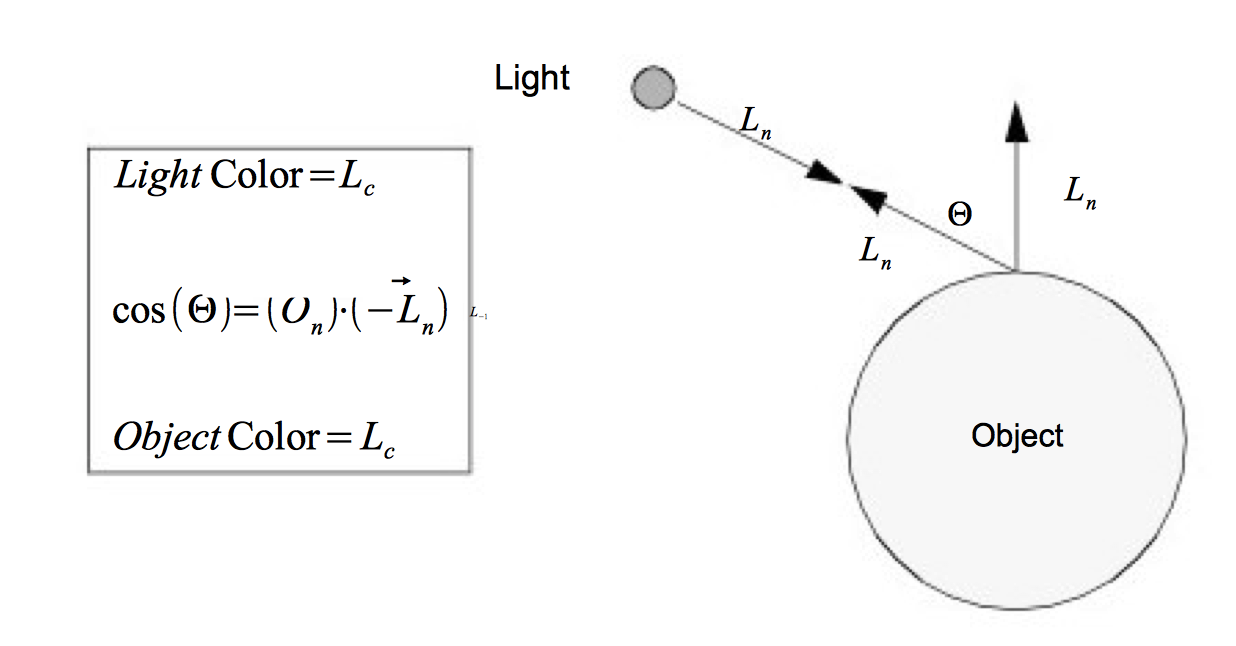
\includegraphics[width=0.8\textwidth]{Figure3-8}\\
  \caption{Diffuse lighting}\label{fig:Figure3-8}
\end{figure}

\begin{figure}[!htb]
  \centering
  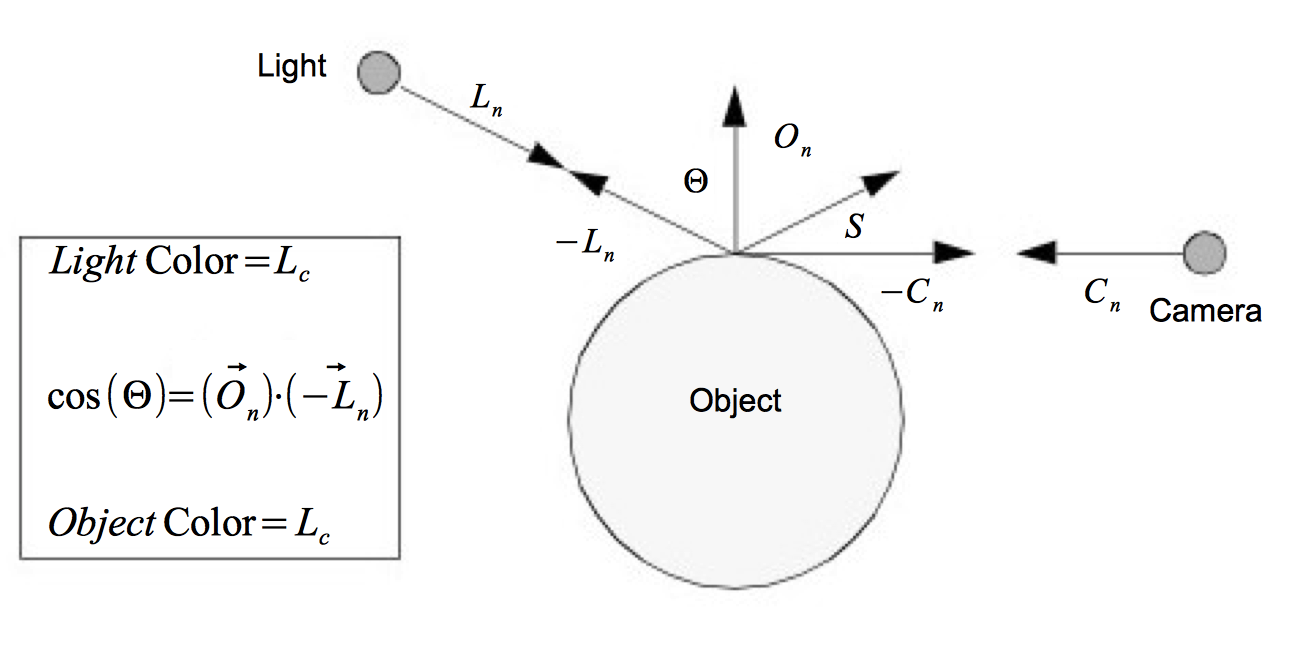
\includegraphics[width=0.8\textwidth]{Figure3-9}\\
  \caption{Specular lighting.}\label{fig:Figure3-9}
\end{figure}

We have presented the equations for the different lighting models independently. We can apply all lighting models simultaneously or in combination. Equation \ref{eq:3.4} combines ambient, diffuse and specular lighting into one equation.

\begin{equation}\label{eq:3.4}
  R_c = O_{ai}O_{ac}L_c - O_{di}O_{dc}L_c(\overrightarrow{O}_n \cdot \overrightarrow{L}_n) + O_{si}O_{sc}L_c[\overrightarrow{S} \cdot(-\overrightarrow{C}_n)]^{O_{sp}}
\end{equation}
\myequations{Ambient, Diffuse and Specular Lighting}


The result is a color at a point on the surface of the object. The constants $O_{ai}$, $O_{di}$, and $O_{si}$ control the relative amounts of ambient, diffuse and specular lighting for an object. The constants $O_{ac}$ $O_{dc}$ and $O_{sc}$ specify the colors to be used for each type of lighting. These six constants along with the specular power are part of the surface material properties. (Other properties such as transparency will be covered in later sections of the text.) Different combinations of these property values can simulate dull plastic and polished metal. The equation assumes an infinite point light source as described in ``Lights'' on \ref{Lights}. However the equation can be easily modified to incorporate other types of directional lighting.

\begin{figure}[!htb]
  \centering
  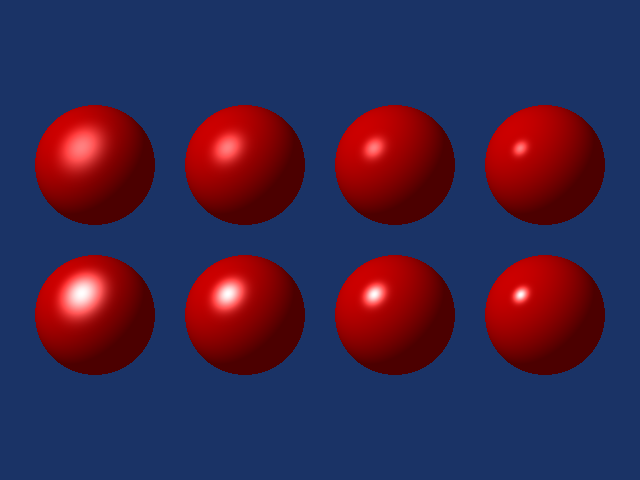
\includegraphics[width=0.8\textwidth]{Figure3-10}\\
  \caption{Effects of specular coefficients. Specular coefficients control the apparent "shininess" of objects. The top row has a specular intensity value of 0.5; the bottom row 1.0. Along the horizontal direction the specular power changes. The values (from left to right) are 5, 10, 20, and 40.}\label{fig:Figure3-10}
\end{figure}
\index{actor!surface properties|)}\index{light|)}\index{surface properties|)}

\section{Cameras}
\label{sec:cameras}
\index{camera|(}

We have light sources that are emitting rays of light and actors with surface properties. At every point on the surface of our actors this interaction results in some composite color (i.e., combined color from light, object surface, specular, and ambient effects). All we need now to render the scene is a camera. There are a number of important factors that determine how a 3D scene gets projected onto a plane to form a 2D image (see Figure \ref{fig:Figure3-11}). These are the position\index{camera!position}, orientation, and focal point\index{camera!focal point} of the camera, the method of camera projection, and the location of the camera \emph{clipping planes}\index{clipping plane}.

\begin{figure}[!htb]
  \centering
  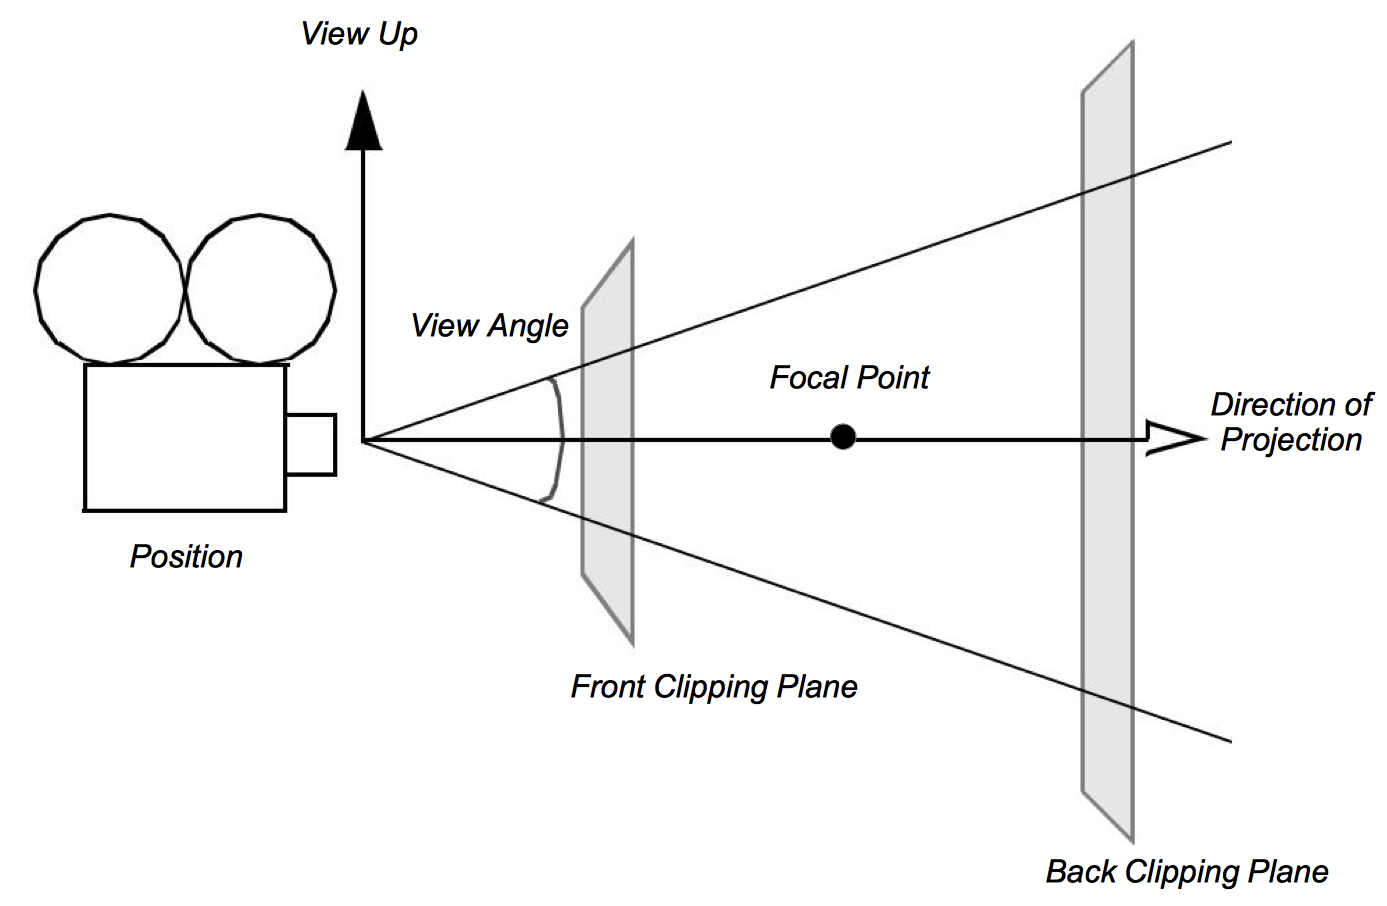
\includegraphics[width=0.8\textwidth]{Figure3-11}\\
  \caption{Camera attributes.}\label{fig:Figure3-11}
\end{figure}

The position and focal point of the camera define the location of the camera and where it points. The vector defined from the camera position to the focal point is called the \emph{direction of projection}\index{direction of projection}. The camera image plane is located at the focal point and is typically perpendicular to the projection vector\index{projection vector}. The camera orientation is controlled by the position and focal point plus the camera view-up vector. Together these completely define the camera view. 

The method of projection controls how the actors are mapped to the image plane. \emph{Orthographic projection}\index{orthographic projection}\index{projection!orthographic} is a parallel mapping process. In orthographic projection (or parallel projection\index{parallel projection}\index{projection!parallel}) all rays of light entering the camera are parallel to the projection vector. \emph{Perspective projection}\index{perspective projection}\index{projection!perspective} occurs when all light rays go through a common point (i.e., the viewpoint or center of projection). To apply perspective projection we must specify a perspective angle or camera view angle.

The front and back clipping planes intersect the projection vector, and are usually perpendicular to it. The clipping planes are used to eliminate data either too close to the camera or too far away. As a result only actors or portions of actors within the clipping planes are (potentially) visible. Clipping planes are typically perpendicular to the direction of projection. Their locations can be set using the camera's clipping range. The location of the planes are measured from the camera's position along the direction of projection. The front clipping plane is at the minimum range value, and the back clipping plane is at the maximum range value. Later on in Chapter 7: \nameref{chap:advanced_computer_graphics}, when we discuss stereo rendering, we will see examples of clipping planes that are not perpendicular to the direction of projection.

Taken together these camera parameters define a rectangular pyramid, with its apex at the camera's position and extending along the direction of projection. The pyramid is truncated at the top with the front clipping plane and at the bottom by the back clipping plane. The resulting view frustum defines the region of 3D space visible to the camera.

While a camera can be manipulated\index{camera!manipulation} by directly setting the attributes mentioned above, there are some common operations that make the job easier. Figure \ref{fig:Figure3-12} and Figure \ref{fig:Figure3-13} will help illustrate these operations. Changing the \emph{azimuth}\index{azimuth}\index{camera!azimuth} of a camera rotates its position around its view up\index{camera!view up} vector, centered at the focal point. Think of this as moving the camera to the left or right while always keeping the distance to the focal point constant. Changing a camera's \emph{elevation}\index{camera!elevation}\index{elevation} rotates its position around the cross product of its direction of projection and view up centered at the focal point. This corresponds to moving the camera up and down. To \emph{roll}\index{camera!roll}\index{roll} the camera, we rotate the view up vector about the view plane normal\index{camera!view plane normal}. Roll is sometimes called twist.

The next two motions keep the camera's position constant and instead modify the focal point. Changing the \emph{yaw}\index{camera!yaw} rotates the focal point about the view up centered at the camera's position. This is like an azimuth, except that the focal point moves instead of the position. Changes in \emph{pitch}\index{camera!pitch}\index{pitch} rotate the focal point about the cross product of the direction of projection and view up centered at the camera's position. \emph{Dollying}\index{camera!dolly}\index{dolly} in and out moves the camera's position along the direction of projection, either closer or farther from the focal point. This operation is specified as the ratio of its current distance to its new distance. A value greater than one will dolly in, while a value less than one will dolly out. Finally, \emph{zooming} changes the camera's view angle, so that more or less of the scene falls within the view frustum.

\begin{figure}[!htb]
  \centering
  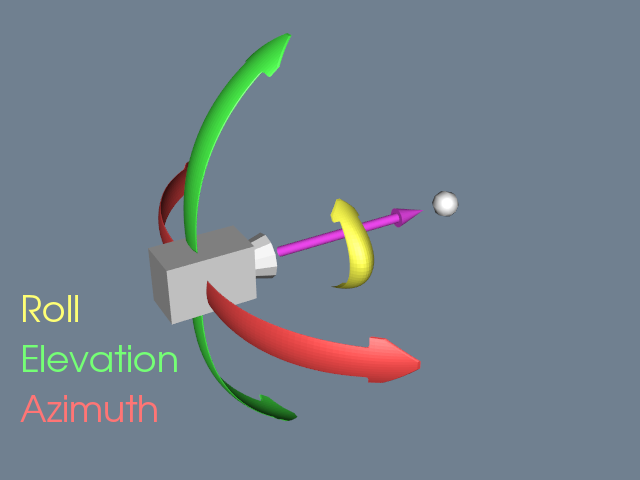
\includegraphics[width=0.8\textwidth]{Figure3-12}\\
  \caption{Camera movements around the focal point.}\label{fig:Figure3-12}
\end{figure}

\begin{figure}[!htb]
  \centering
  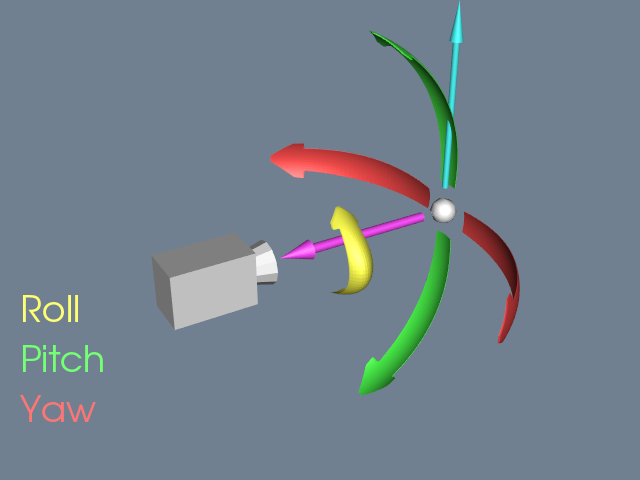
\includegraphics[width=0.8\textwidth]{Figure3-13}\\
  \caption{Camera movements around the camera position.}\label{fig:Figure3-13}
\end{figure}

Once we have the camera situated, we can generate our 2D image. Some of the rays of light traveling through our 3D space will pass through the lens on the camera. These rays then strike a flat surface to produce an image. This effectively projects our 3D scene into a 2D image. The camera's position and other properties determine which rays of light get captured and projected. More specifically, only rays of light that intersect the camera's position, and are within its viewing frustum, will affect the resulting 2D image.

This concludes our brief rendering overview. The light has traveled from its sources to the actors, where it is reflected and scattered. Some of this light gets captured by the camera and produces a 2D image. Now we will look at some of the details of this process.
\index{camera|)}

\section{Coordinate Systems}
\label{sec:coordinate_systems}

There are four coordinate systems commonly used in computer graphics and two different ways of representing points within them (Figure \ref{fig:Figure3-14}). While this may seem excessive, each one serves a purpose. The four coordinate systems we use are: \emph{model}, \emph{world} , \emph{view}, and \emph{display}.

The model\index{coordinate system!model}\index{model coordinate system} coordinate system is the coordinate system in which the model is defined, typically a local Cartesian coordinate system. If one of our actors represents a football, it will be based on a coordinate system natural to the football geometry (e.g., a cylindrical system). This model has an inherent coordinate system determined by the decisions of whoever generated it. They may have used inches or meters as their units, and the football may have been modelled with any arbitrary axis as its major axis.

The world\index{coordinate system!world} coordinate system is the 3D space in which the actors are positioned. One of the actor's responsibilities is to convert from the model's coordinates into world coordinates. Each model may have its own coordinate system but there is only one world coordinate system. Each actor must scale, rotate, and translate its model into the world coordinate system. (It may also be necessary for the modeller to transform from its natural coordinate system into a local Cartesian system. This is because actors typically assume that the model coordinate system is a local Cartesian system.) The world coordinate system is also the system in which the position and orientation of cameras and lights are specified.

The view\index{coordinate system!view}\index{view coordinate system} coordinate system represents what is visible to the camera. This consists of a pair of x and y values, ranging between $(-1,1)$, and a \emph{z} depth coordinate. The \emph{x}, \emph{y} values specify location in the image plane, while the \emph{z} coordinate represents the distance, or range, from the camera. The camera's properties are represented by a four by four transformation matrix\index{transformation matrix} (to be described shortly), which is used to convert from world coordinates into view coordinates. This is where the perspective effects of a camera are introduced.

The display coordinate system\index{coordinate system!display}\index{display coordinate system} uses the same basis as the view coordinate system, but instead of using negative one to one as the range, the coordinates are actual \emph{x}, \emph{y} pixel locations on the image plane. Factors such as the window's size on the display determine how the view coordinate range of $(-1,1)$ is mapped into pixel locations. This is also where the viewport comes into effect.

\begin{figure}[!htb]
  \centering
  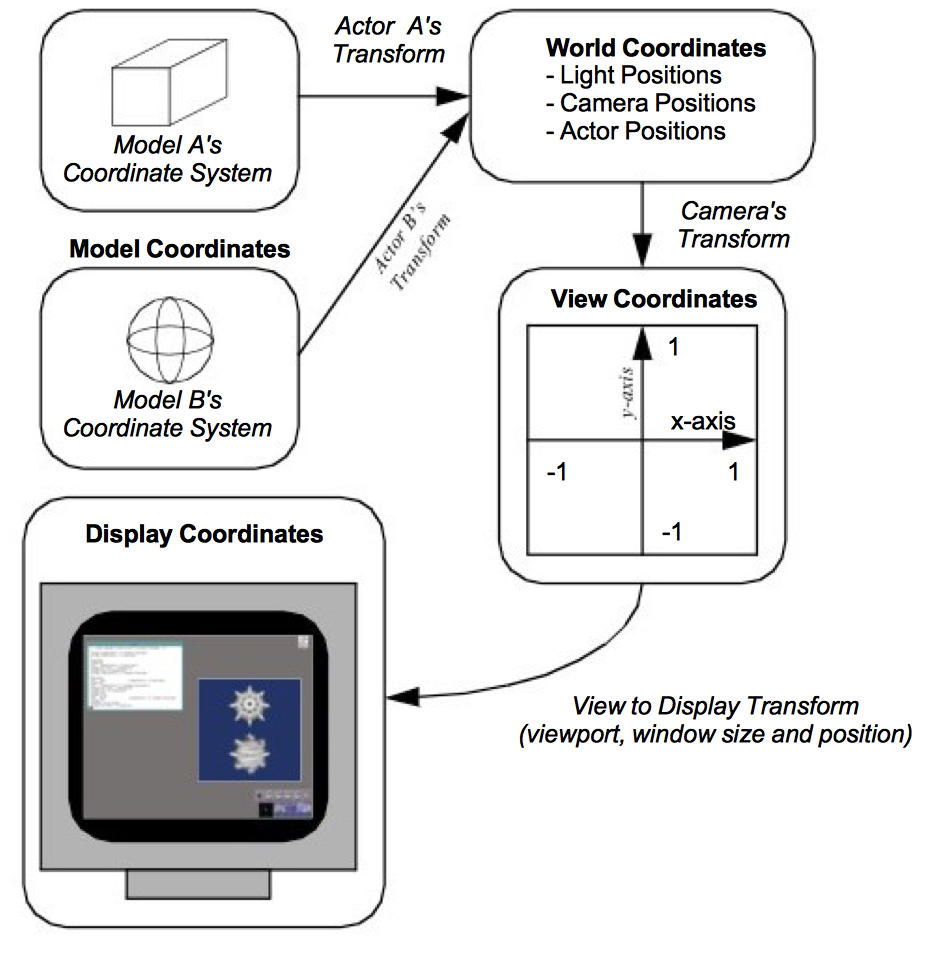
\includegraphics[width=0.8\textwidth]{Figure3-14}\\
  \caption{ Modelling, world, view and display coordinate system.}\label{fig:Figure3-14}
\end{figure}

You may want to render two different scenes, but display them in the same window. This can be done by dividing the window into rectangular viewports. Then, each renderer can be told what portion of the window it should use for rendering. The viewport ranges from $(0,1)$ in both the \emph{x} and \emph{y} axis. Similar to the view coordinate system, the \emph{z}--value in the display coordinate system also represents depth into the window. The meaning of this \emph{z}--value will be further described in the section titled ``Z-Buffer'' on page \pageref{Z-Buffer}.


\section{Coordinate Transformation}
\index{transformation!coordinate|(}

When we create images with computer graphics, we project objects defined in three dimensions onto a two--dimensional image plane. As we saw earlier, this projection naturally includes perspective. To include projection effects such as vanishing points we use a special coordinate system called \emph{homogeneous coordinates}\index{homogeneous coordinates}.

The usual way of representing a point\index{point!transformation} in 3D is the three element Cartesian vector $(x, y, z)$. Homogeneous coordinates are represented by a four element vector $( x_hh, y_h, z_h, w_h )$. The conversion between Cartesian coordinates and homogeneous coordinates is given by:

\begin{equation}\label{eq:3.5}
x = \frac{x_h}{w_h}\ \ \ \  x = \frac{y_h}{w_h}\ \ \ \ x = \frac{z_h}{w_h}
\end{equation}
\myequations{Cartesian to Homogenous Conversion}

Using homogeneous coordinates we can represent an infinite point by setting w h to zero. This capability is used by the camera for perspective transformations. The transformations are applied by using a 4x4 transformation matrix . Transformation matrices\index{transformation matrix} are widely used in computer graphics because they allow us to perform translation, scaling, and rotation of objects by repeated matrix multiplication. Not all of these operations can be performed using a 3x3 matrix.

For example, suppose we wanted to create a transformation matrix\index{transformation matrix!translation} that translates a point $( x, y, z)$ in Cartesian space by the vector $( t_x , t_y, t_z)$. We need only construct the translation matrix given by

\begin{equation}\label{eq:3.6}
T_T = \left[\begin{array}{cccc}
1 & 0 & 0 & t_x       \\
0 & 1 & 0 & t_y      \\
0 & 0 & 1 & t_z      \\
0 & 0 & 0 & 1
\end{array}\right]
\end{equation}
\myequations{Translation}

and then postmultiply it with the homogeneous coordinate $(x_h, y_h, z_h, w_h)$. To carry this example through, we construct the homogeneous coordinate from the Cartesian coordinate $( x, y, z)$ by setting $w_h = 1$ to yield $(x, y, z, 1)$. Then to determine the translated point $(x' , y', z')$ we premultiply current position by the transformation matrix $T_T$ to yield the translated coordinate. Substituting into Equation \ref{eq:3.6} we have the result

\begin{equation}\label{eq:3.7}
\left[\begin{array}{c}
x'      \\
y'       \\
z'      \\
w'
\end{array}\right] =\left[\begin{array}{cccc}
1 & 0 & 0 & t_x       \\
0 & 1 & 0 & t_y       \\
0 & 0 & 1 & t_z      \\
0 & 0 & 0 & 1
\end{array}\right] \cdot
\left[\begin{array}{c}
x      \\
y       \\
z      \\
1
\end{array}\right] 
\end{equation}

Converting back to Cartesian coordinates via Equation \ref{eq:3.5} we have the expected solution

\begin{equation}\label{eq:3.8}
x' = x +t_x \\
y' = y + t_y \\
z' = z + t_z
\end{equation}
\myequations{Homogenous to Cartesian}

The same procedure is used to scale or rotate an object. To scale an object we use the transformation matrix\index{transformation matrix!scaling}

\begin{equation}\label{eq:3.9}
T_s = \left[\begin{array}{cccc}
s_x & 0 & 0 & 0 \\
0 & s_y & 0 & 0 \\
0 & 0 & s_z & 0 \\
0 & 0 & 0 & 1
\end{array}\right]
\end{equation}
\myequations{Scaling}


where the parameters $s_x, s_y$, and $s_z$ are scale factors along the $x, y, z$ axes. Similarly we can rotate an object around the $x$ axes by angle $\theta$ using the matrix\index{transformation matrix!rotation}

\begin{equation}\label{eq:3.10}
T_{R_x} = \left[\begin{array}{cccc}
1 & 0 & 0 & 0 \\
0 & \cos\theta & -\sin\theta & 0 \\
0 & \sin\theta & \cos\theta & 0 \\
0 & 0 & 0 & 1
\end{array}\right]
\end{equation}
\myequations{$X-$axis rotation }


Around the $y$ axis we use

\begin{equation}\label{eq:3.11}
TT_{R_y} = \left[\begin{array}{cccc}
\cos\theta & 0 & \sin\theta0 & 0 \\
0 & 1 & 0 & 0 \\
-\sin\theta & 0 & \cos\theta & 0 \\
0 & 0 & 0 & 1
\end{array}\right]
\end{equation}
\myequations{$Y-$axis rotation }

and around the $z$ axis we use

\begin{equation}\label{eq:3.12}
T_{R_z} = \left[\begin{array}{cccc}
\cos\theta & -\sin\theta & 0 & 0 \\
\sin\theta & \cos\theta & 0 & 0 \\
0 & 0 & 0 & 0 \\
0 & 0 & 0 & 1
\end{array}\right]
\end{equation}
\myequations{$Z-$axis rotation }

Another useful rotation matrix is used to transform one coordinate axes $x-y-z$ to another coordinate axes $x'-y'-z'$. To derive the transformation matrix we assume that the unit $x'$. To derive the transformation matrix we assume that the unit $x'$ axis make the angles $(\theta_{x'x},\theta_{x'y},\theta_{x'z})$ around the x-y-z axes (these are called direction cosines\index{direction cosine}). Similarly, the unit $y'$ axis makes the angles $(\theta_{y'x},\theta_{y'y},\theta_{y'z})$ and the unit $z'$ axis makes the angles $(\theta_{z'x},\theta_{z'y},\theta_{z'z})$. The resulting rotation matrix is formed by placing the direction cosines along the rows of the transformation matrix as follows

\begin{equation}\label{eq:3.13}
T_R = \left[\begin{array}{cccc}
\cos\theta_{x'x} & \cos\theta_{x'y} & \cos\theta_{x'z} & 0 \\
\cos\theta_{y'x} & \cos\theta_{z'y} & \cos\theta_{y'z} & 0 \\
\cos\theta_{z'x} & \cos\theta_{z'y} & \cos\theta_{z'z} & 0 \\
0 & 0 & 0 & 1
\end{array}\right]
\end{equation}
\myequations{Transform from $(x,y,z)$ to $(x',y',z')$ }


Rotations occur about the coordinate origin. It is often more convenient to rotate around the center of the object (or a user-specified point). Assume that we call this point the object's center . To rotate around we Oc must first translate the object to the Oorigin, apply rotations, and then translate the object back.

Transformation matrices can be combined by matrix multiplication to achieve combinations of translation, rotation, and scaling. It is possible for a single transformation matrix to represent all types of transformation simultaneously. This matrix is the result of repeated matrix multiplications. A word of warning: The order of the multiplication is important. For example, multiplying a translation matrix by a rotation matrix will not yield the same result as multiplying the rotation matrix by the translation matrix.
\index{transformation!coordinate|)}

\section{Actor Geometry}
\index{actor!geometry|(}

We have seen how lighting properties control the appearance of an actor, and how the camera in combination with transformation matrices is used to project an actor to the image plane. What is left to define is the geometry of the actor, and how we position it in the world coordinate system.

\subsection{Modelling}

A major topic in the study of computer graphics is modelling or representing the geometry of physical objects. Various mathematical techniques have been applied including combinations of points, lines, polygons, curves, and splines of various forms, and even implicit mathematical functions.

This topic is beyond the scope of the text. The important point here is that there is an underlying geometric model that specifies what the object's shape is and where it is located in the model coordinate system.

In data visualization, modelling takes a different role. Instead of directly creating geometry to represent an object, visualization algorithms \emph{compute} these forms. Often the geometry is abstract (like a contour line) and has little relationship to real world geometry. We will see how these models are computed when we describe visualization algorithms in Chapter 6: \nameref{chap:fundamental_algorithms} and Chapter 9: \nameref{chap:advanced_algorithms}.

The representation of geometry for data visualization tends to be simple, even though computing the representations is not. These forms are most often primitives like points, lines, and polygons, or visualization data such as volume data. We use simple forms because we desire high performance and interactive systems. Thus we take advantage of computer hardware (to be covered in ``Graphics Hardware'' on \ref{sec:graphics_hardware} ) or special rendering techniques like volume rendering (see ``Volume Rendering'' on \ref{sec:volume_rendering} ).

\subsection{Actor Location and Orientation}

Every actor has a transformation matrix that controls its location and scaling in world space. The actor's geometry is defined by a model in model coordinates. We specify the actor's location using orientation, position, and scale factors along the coordinate axes. In addition, we can define an origin around which the actor rotates. This feature is useful because we can rotate the actor around its center or some other meaningful point.

The orientation of an actor is determined by rotations stored in an orientation vector (Ox,Oy, Oz). This vector defines a series of rotational transformation matrices. As we saw in the previous section on transformation matrices, the order of application of the transformations is not arbitrary. We have chosen a fixed order based on what we think is natural to users. The order of transformation is a rotation by O y around the y axis, then by around Ox the x axis, and finally by O z around the z axis. This ordering is arbitrary and is based on the standard camera operations. These operations (in order) are a camera azimuth, followed by an elevation, and then a roll (Figure\ref{fig:Figure3-15}).

All of these rotations take place around the origin of the actor. Typically this is set to the center of its bounding box, but it can be set to any convenient point. There are many different methods for changing an actor's orientation. RotateX(), RotateY(), and RotateZ() are common methods that rotate about their respective axes. Many systems also include a method to rotate about a userdefined axis. In the Visualization Toolkit the RotateXYZ() method is used to rotate around an arbitrary vector passing through the origin.

\begin{figure}[!htb]
  \centering
  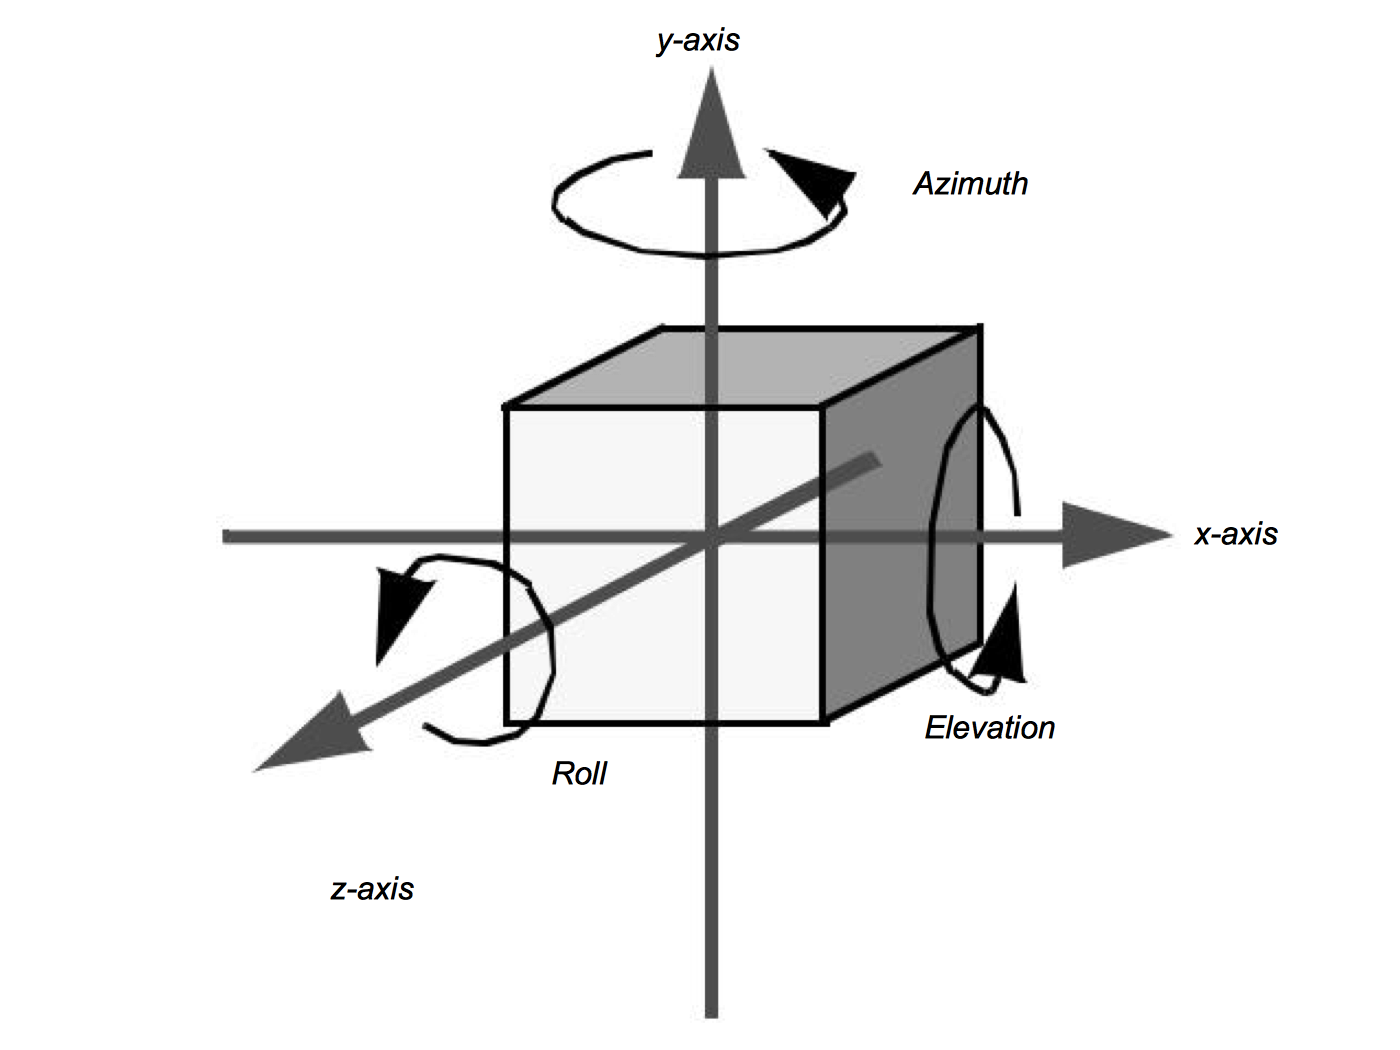
\includegraphics[width=0.8\textwidth]{Figure3-15}\\
  \caption{Actor coordinate system.}\label{fig:Figure3-15}
\end{figure}

\index{actor!geometry|)}

\section{Graphics Hardware}
\label{sec:graphics_hardware}
\index{graphics hardware|(}\index{hardware|(}

Earlier we mentioned that advances in graphics hardware have had a large impact on how rendering is performed. Now that we have covered the fundamentals of rendering a scene, we look at some of the hardware issues. First, we discuss raster devices that have replaced vector displays as the primary output device. Then, we look at how our programs communicate to the graphics hardware. We also examine the different coordinate systems used in computer graphics, hidden line/surface removal, and \emph{z}-buffering.

\subsection{Raster Devices}
\label{subsec:rasterization}
\index{raster hardware|(}

The results of computer graphics is pervasive in today's world---digital images (generated with computer graphics) may be found on cell phones, displayed on computer monitors, broadcast on TV, shown at the movie theatre and presented on electronic billboards. All of these, and many more, display mediums are raster devices. A raster device represents an image using a two dimensional array of picture elements called pixels\index{pixel}. For example, the word "hello" can be represented as an array of pixels. as shown in Figure \ref{fig:Figure3-16}. Here the word "hello" is written within a pixel array that is twenty-five pixels wide and ten pixels high. Each pixel stores one bit of information, whether it is black or white. This is how a black and white laser printer works, for each point on the paper it either prints a black dot or leaves it the color of the paper. Due to hardware limitations, raster devices such as laser printers and computer monitors do not actually draw accurate square pixels like those in Figure \ref{fig:Figure3-16}. Instead, they tend to be slightly blurred and overlapping. Another hardware limitation of raster devices is their resolution. This is what causes a 300 dpi (dots per inch) laser printer to produce more detailed output than a nine pin dot matrix printer. A 300 dpi laser printer has a resolution of 300 pixels per inch compared to roughly 50 dpi for the dot matrix printer.

\begin{figure}[!htb]
  \centering
  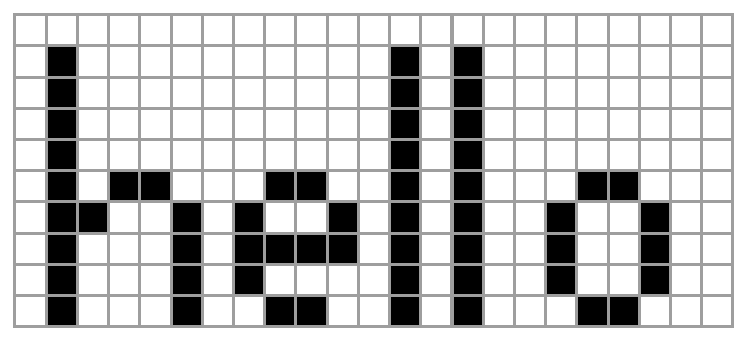
\includegraphics[width=0.8\textwidth]{Figure3-16}\\
  \caption{A pixel array for the word "hello".}\label{fig:Figure3-16}
\end{figure}

Color computer monitors typically have a resolution of about 80 pixels per inch, making the screen a pixel array roughly one thousand pixels in width and height. This results in over one million pixels, each with a value that indicates what color it should be. Since the hardware in color monitors uses the RGB\index{RGB} system, it makes sense to use that to describe the colors in the pixels. Unfortunately, having over one million pixels, each with a red, green, and blue component, can take up a lot of memory. This is part of what differentiates the variety of graphics hardware on the market. Some companies use 24 bits of storage per pixel, others use eight, some advanced systems use more than 100 bits of storage per pixel. Typically, the more bits per pixel the more accurate the colors will be.

\begin{figure}[!htb]
  \centering
  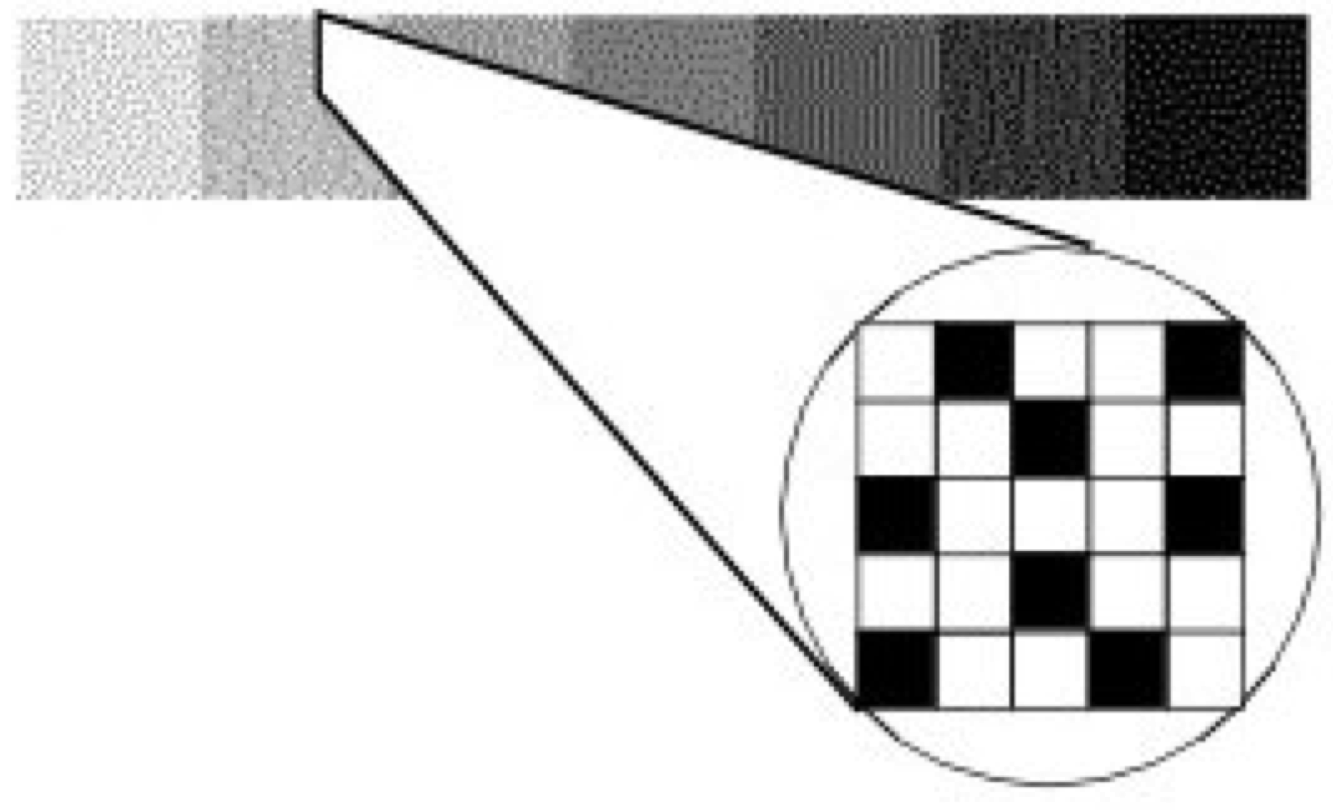
\includegraphics[width=0.8\textwidth]{Figure3-17}\\
  \caption{Black and white dithering.}\label{fig:Figure3-17}
\end{figure}

One way to work around color limitations in the graphics hardware is by using a technique called \emph{dithering}\index{dithering}. Say, for example, that you want to use some different shades of gray, but your graphics hardware only supports black and white. Dithering lets you approximate shades of gray by using a mixture of both black and white pixels. In Figure \ref{fig:Figure3-17}, seven gray squares are drawn using a mixture of black and white pixels. From a distance the seven squares look like different shades of gray even though up close, it's clear that they are just different mixtures of black and white pixels. This same technique works just as well for other colors. For example, if your graphics hardware supports primary blue, primary green, and white but not a pastel sea green, you can approximate this color by dithering the green, blue, and white that the hardware does support.
\index{raster hardware|)}


\subsection{Interfacing to the Hardware}

Now that we have covered the basics of display hardware, the good news is that you rarely need to worry about them. Most graphics programming is done using higher-level primitives than individual pixels. Figure \ref{fig:Figure3-18} shows a typical arrangement for a visualization program. At the bottom of the hierarchy is the display hardware that we already discussed; chances are your programs will not interact directly with it. The top three layers above the hardware are the layers you may need to be concerned with.

\begin{figure}[!htb]
  \centering
  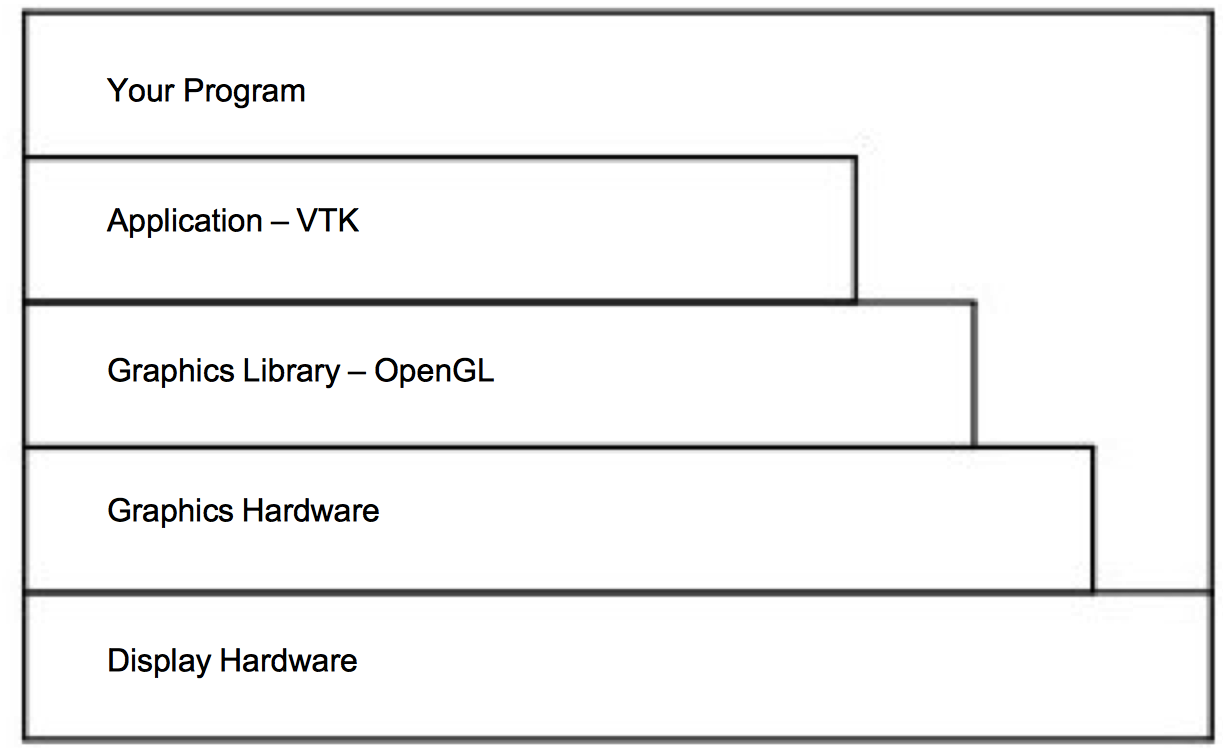
\includegraphics[width=0.8\textwidth]{Figure3-18}\\
  \caption{Typical graphics interface hierarchy.}\label{fig:Figure3-18}
\end{figure}

Many programs take advantage of application libraries as a high-level interface to the graphics capabilities of a system. The \emph{Visualization Toolkit} accompanying this book is a prime example of this. It allows you to display a complex object or graph using just a few commands. It is also possible to interface to a number of different graphics libraries, since different libraries may be supported on different hardware platforms.

The graphics library and graphics hardware layers both perform similar functions. They are responsible for taking high-level commands from an application library or program, and executing them. This makes programming much easier by providing more complex primitives to work with. Instead of drawing pixels one at a time, we can draw primitives like polygons, triangles, and lines, without worrying about the details of which pixels are being set to which colors. Figure \ref{fig:Figure3-19} illustrates some high-level primitives that all mainstream graphics libraries support.

This functionality is broken into two different layers because different machines may have vastly different graphics hardware. If you write a program that draws a red polygon, either the graphics library or the graphics hardware must be able to execute that command. On high-end systems, this may be done in the graphics hardware, on others it will be done by the graphics library in software. So the same commands can be used with a wide variety of machines, without worrying about the underlying graphics hardware.

\begin{figure}[!htb]
  \centering
  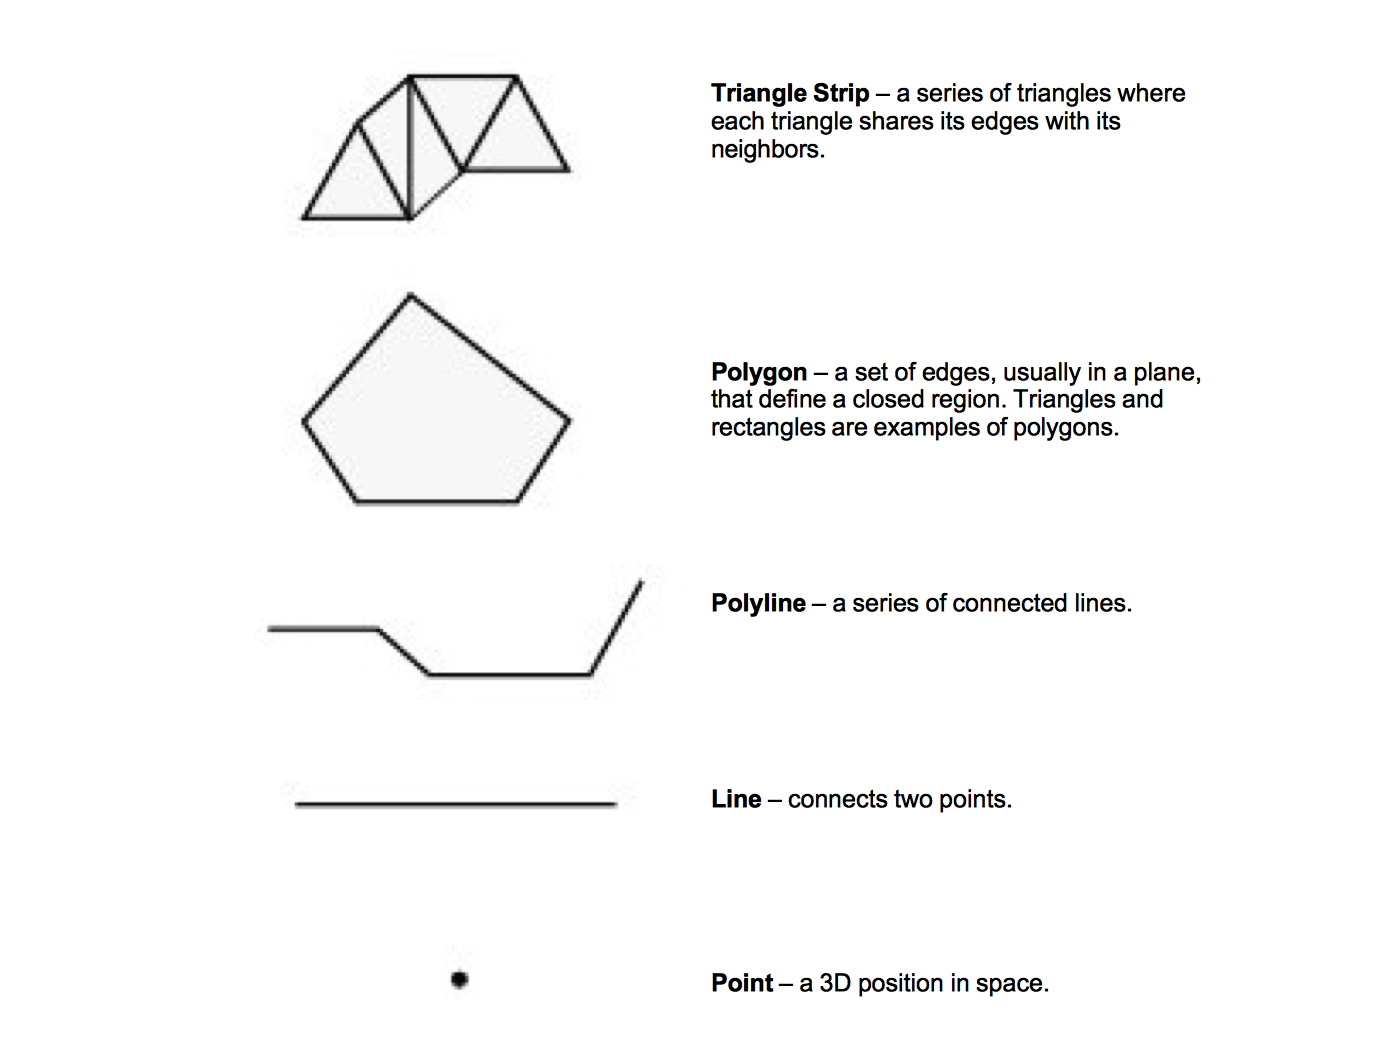
\includegraphics[width=0.8\textwidth]{Figure3-19}\\
  \caption{Graphics primitives.}\label{fig:Figure3-19}
\end{figure}

The fundamental building block of the primitives in Figure \ref{fig:Figure3-19} is a point\index{point} (or vertex). A vertex\index{vertex} has a position, normal, and color, each of which is a three element vector. The position specifies where the vertex is located, its normal specifies which direction the vertex is facing, and its color specifies the vertex's red, green, and blue components.

A polygon\index{polygon} is built by connecting a series of points or vertices as shown in Figure \ref{fig:Figure3-20}. You may be wondering why each vertex has a normal, instead of having just one normal for the entire polygon. A planar polygon can only be facing one direction regardless of what the normals of its vertices indicate. The reason is that sometimes a polygon is used as an approximation of something else, like a curve. Figure \ref{fig:Figure3-21} shows a top-down view of a cylinder. As you can see, it's not really a cylinder but rather a polygonal approximation of the cylinder drawn in gray. Each vertex is shared by two polygons and the correct normal for the vertex is not the same as the normal for the polygon. Similar logic explains why each vertex has a color instead of just having one color for an entire polygon.

When you limit yourself to the types of primitives described above, there are some additional properties that many graphics systems support. Edge color and edge visibility can be used to highlight the polygon primitives that make up an actor. Another way to do this is by adjusting the representation from \emph{surface} to \emph{wireframe} or \emph{points}. This replaces surfaces such as polygons with either their boundary edges or points respectively. While this may not make much sense from a physical perspective, it can help in some illustrations. Using edge visibility when rendering a CAD model can help to show the different pieces that comprise the model.

\subsection{Rasterization}
\index{rasterization|(}

At this point in the text we have described how to represent graphics data using rendering primitives, and we have described how to represent images using raster display devices. The question remains, how do we convert graphics primitives into a raster image? This is the topic we address in this section. Although a thorough treatise on this topic is beyond the scope of this text, we will do our best to provide a high-level overview.

\begin{figure}[!htb]
  \centering
  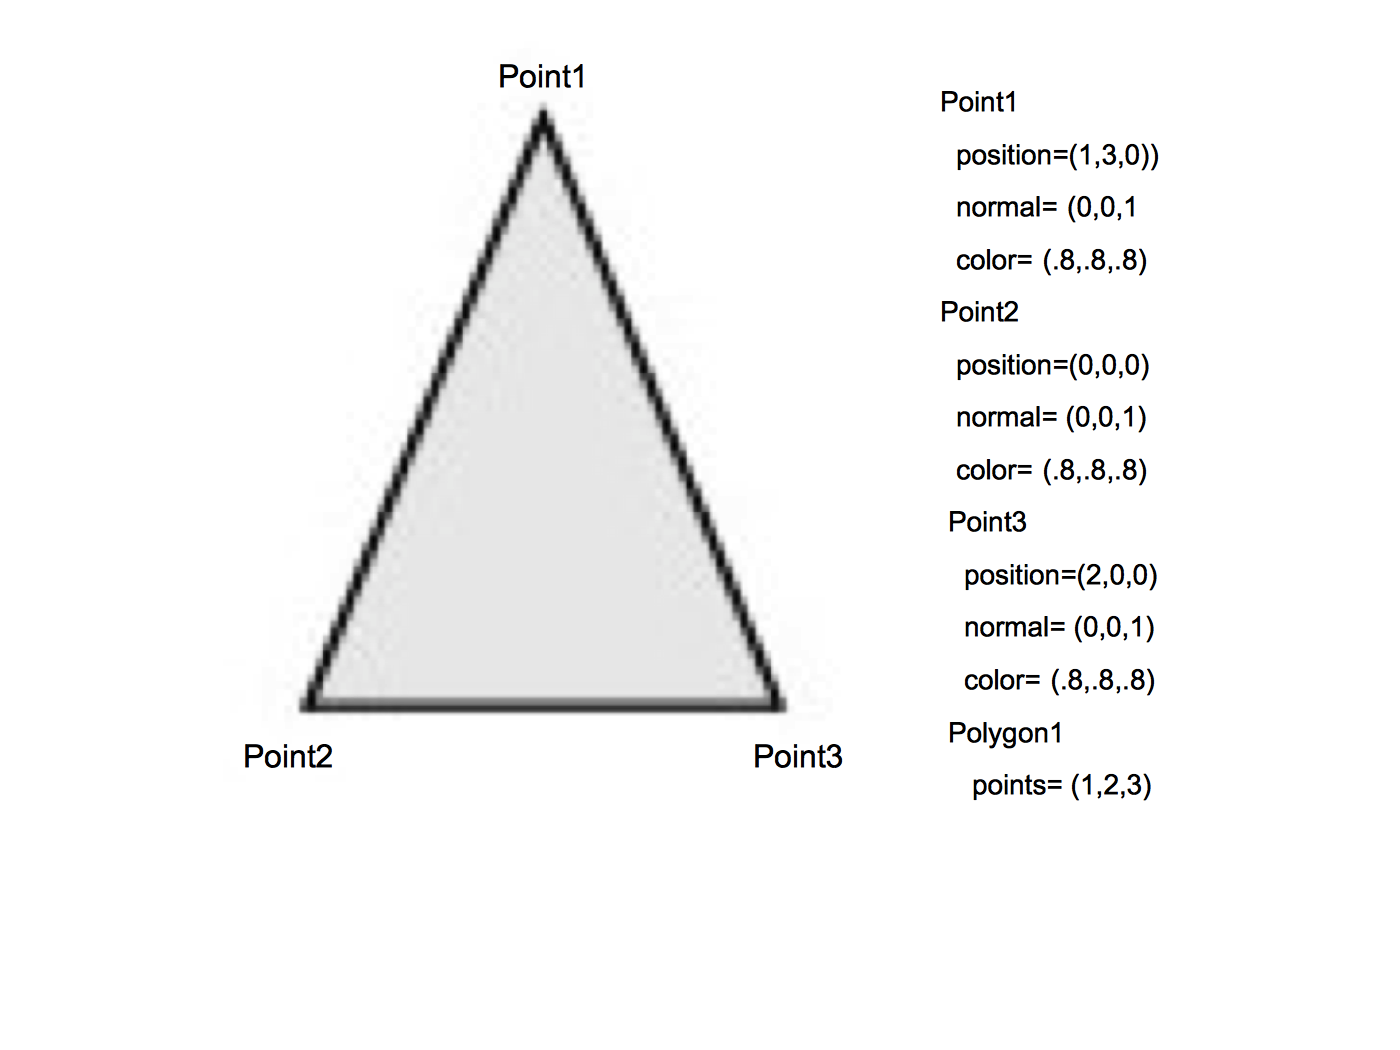
\includegraphics[width=0.8\textwidth]{Figure3-20}\\
  \caption{An example polygon.}\label{fig:Figure3-20}
\end{figure}

\begin{figure}[!htb]
  \centering
  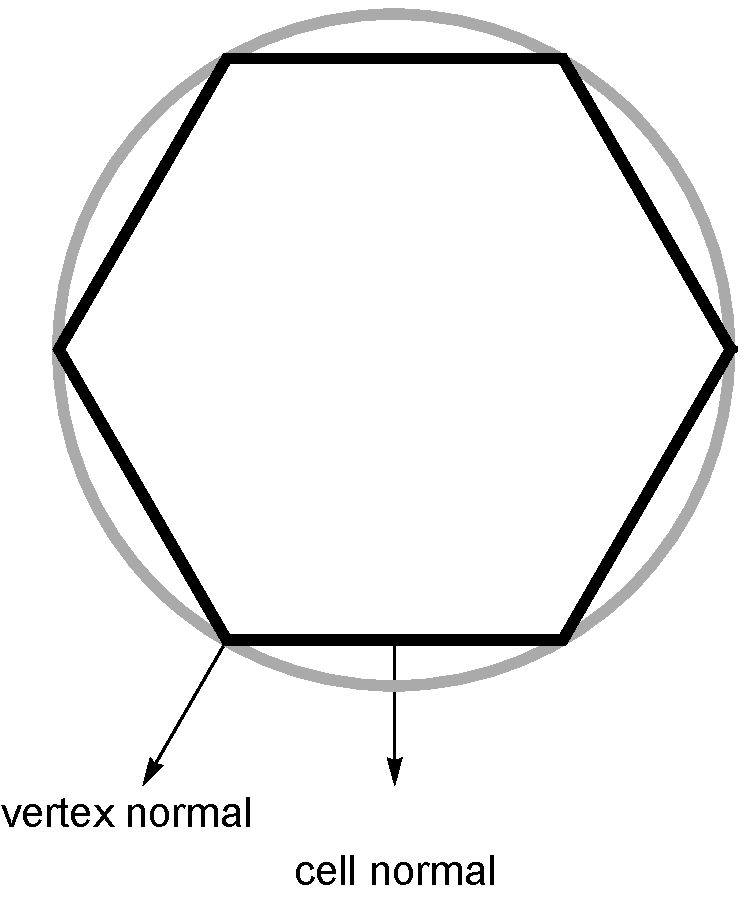
\includegraphics[width=0.8\textwidth]{Figure3-21}\\
  \caption{Vertex and polygon normals.}\label{fig:Figure3-21}
\end{figure}

The process of converting a geometric representation into a raster image is called \emph{rasterization} or \emph{scan conversion}. In the description that follows we assume that the graphics primitives are triangle polygons. This is not as limiting as you might think, because any general polygon can be tessellated into a set of triangles. Moreover, other surface representations such as splines are usually tessellated by the graphics system into triangles or polygons. (The method described here is actually applicable to convex polygons.)

Most of today's hardware is based on object-order rasterization techniques. As we saw earlier in this chapter, this means processing our actors in order. And since our actors are represented by polygon primitives, we process polygons one at a time. So although we describe the processing of one polygon, bear in mind that many polygons and possibly many actors are processed.

The first step is to transform the polygon using the appropriate transformation matrix. We also project the polygon to the image plane using either parallel or orthographic projection. Part of this process involves clipping the polygons. Not only do we use the front and back clipping planes to clip polygons too close or too far, but we must also clip polygons crossing the boundaries of the image plane. Clipping polygons that cross the boundary of the view frustum means we have to generate new polygonal boundaries.

\begin{figure}[!htb]
  \centering
  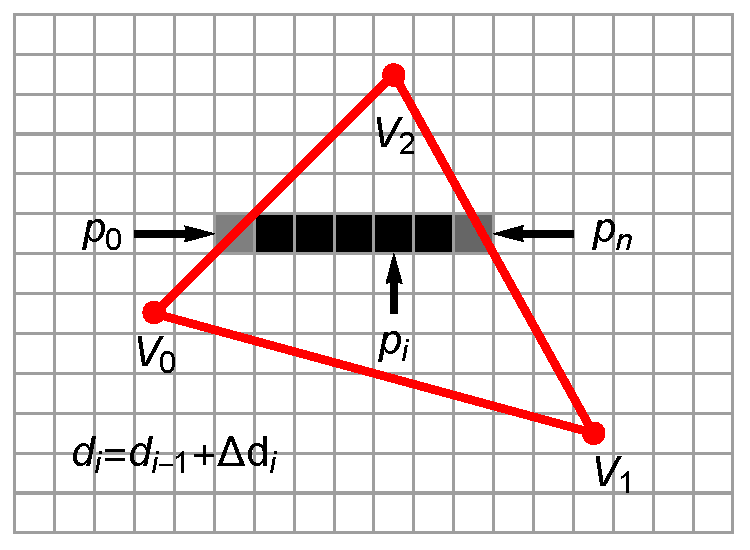
\includegraphics[width=0.8\textwidth]{Figure3-22}\\
  \caption{Rasterizing a convex polygon. Pixels are processed in horizontal spans (or scan-lines) in the image plane. Data values $d_i$ at point $p_i$ are interpolated along the edges and then along the scan-line using delta data values. Typical data values are RGB components of color.}\label{fig:Figure3-22}
\end{figure}

With the polygon clipped and projected to the image plane, we can begin scan-line processing (Figure \ref{fig:Figure3-22}). The first step identifies the initial scan-line intersected by the projected polygon. This is found by sorting the vertices' \emph{y} values. We then find the two edges joining the vertex on the left and right sides. Using the slopes of the edges along with the data values we compute delta data values. These data are typically the \emph{R}, \emph{G}, and \emph{B} color components. Other data values include transparency values and \emph{z} depth values. (The \emph{z} values are necessary if we are using a \emph{z}-buffer, described in the next section.) The row of pixels within the polygon (i.e., starting at the left and right edges) is called a \emph{span}. Data values are interpolated from the edges on either side of the span to compute the internal pixel values. This process continues span-by-span, until the entire polygon is filled. Note that as new vertices are encountered, it is necessary to recompute the delta data values.

The shading\index{SetInputConnection()!shading|(} of the polygon (i.e., color interpolation across the polygon) varies depending on the actor's interpolation attribute. \label{subsection:rasterization.phong}
There are three possibilities: \emph{flat}\index{SetInputConnection()!flat}, \emph{Gouraud}\index{Gouraud shading}\index{SetInputConnection()!Gouraud}, or \emph{Phong shading}\index{Phong shading}\index{SetInputConnection()!Phong}. Figure \ref{fig:Figure3-7} illustrates the difference between flat and Gouraud interpolation. Flat shading\index{flat shading} calculates the color of a polygon by applying the lighting equations to just one normal (typically the surface normal) of the polygon. Gouraud shading calculates the color of a polygon at all of its vertices using the vertices' normals and the standard lighting equations. The interior and edges of the poly-gon are then filled in by applying the scan-line interpolation process. Phong shading is the most realistic of the three. It calculates a normal at every location on the polygon by interpolating the vertex normals. These are then used in the lighting equations to determine the resulting pixel colors. Both flat and Gouraud shading are commonly used methods. The complexity of Phong shading has prevented it from being widely supported in hardware.
\index{SetInputConnection()!shading|)}
\index{rasterization|)}

\subsection{Z-Buffer}
\label{Z-Buffer}

In our earlier description of the rendering process, we followed rays of light from our eye through a pixel in the image plane to the actors and back to the light source. A nice side effect of ray tracing is that viewing rays strike the first actor they encounter and ignore any actors that are hidden behind it. When rendering actors using the polygonal methods described above, we have no such method of computing which polygons are hidden and which are not. We cannot generally count on the polygons being ordered correctly. Instead, we can use a number of hidden-surface methods for polygon rendering.

One method is to sort all of our polygons from back to front (along the camera's view vector) and then render them in that order. This is called the painter's algorithm\index{painter's algorithm} or painter's sort, and has one major weakness illustrated in Figure \ref{fig:Figure3-23}. Regardless of the order in which we draw these three triangles, we cannot obtain the desired result, since each triangle is both in front of, and behind, another triangle. There are algorithms that sort and split polygons as necessary to treat such a situation [Carlson85]. This requires more initial processing to perform the sorting and splitting. If the geometric primitives change between images or the camera view changes, then this processing must be performed before each render.

\begin{figure}[!htb]
  \centering
  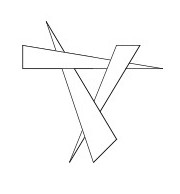
\includegraphics[width=0.8\textwidth]{Figure3-23}\\
  \caption{Problem with Painter's algorithm.}\label{fig:Figure3-23}
\end{figure}

Another hidden surface algorithm, z-buffering, takes care of this problem and does not require sorting. Z-buffering takes advantage of the z-value (i.e., depth value along direction of projection) in the view coordinate system. Before a new pixel is drawn, its z-value is compared against the current z-value for that pixel location. If the new pixel would be in front of the current pixel, then it is drawn and the z-value for that pixel location is updated. Otherwise the current pixel remains and the new pixel is ignored. Z-buffering has been widely implemented in hardware because of its simplicity and robustness. The downside to z-buffering is that it requires a large amount of memory, called a z-buffer, to store a z-value of every pixel. Most systems use a z-buffer with a depth of 24 or 32 bits. For a 1000 by 1000 display that translates into three to four megabytes just for the z-buffer. Another problem with z-buffering is that its accuracy is limited depending on its depth. A 24-bit z-buffer yields a precision of one part in 16,777,216 over the height of the viewing frustum. This resolution is often insufficient if objects are close together. If you do run into situations with z-buffering accuracy, make sure that the front and back clipping planes are as close to the visible geometry as possible.
\index{graphics hardware|)}\index{hardware|)}

\section{Putting It All Together}
This section provides an overview of the graphics objects and how to
use them in VTK.

\subsection{The Graphics Model}

\begin{figure}[!htb]
  \centering
  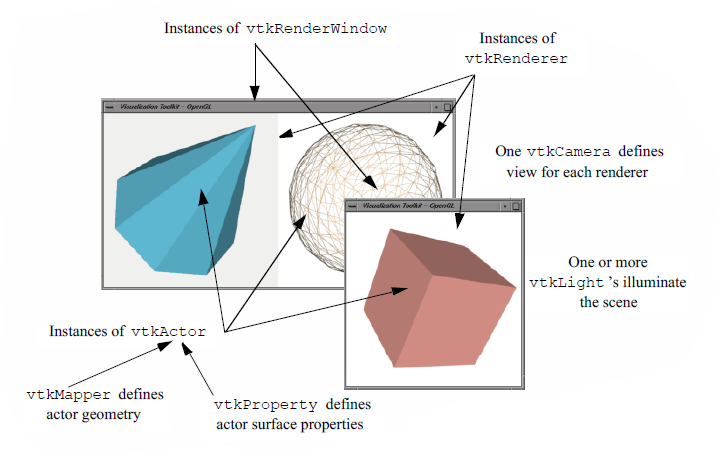
\includegraphics[width=0.8\textwidth]{Figure3-24}\\
  \caption{Illustrative diagram of graphics objects (\href{https://lorensen.github.io/VTKExamples/site/Cxx/Rendering/Model/}{Model.cxx}) and (\href{https://lorensen.github.io/VTKExamples/site/Python/Rendering/Model/}{Model.py}).}\label{fig:Figure3-24}
\end{figure}

We have discussed many of the objects that play a part in the rendering of a scene. Now it's time to put them together into a comprehensive object model for graphics and visualization.

In the \emph{Visualization Toolkit} there are seven basic objects that we use to render a scene. There are many more objects behind the scenes, but these seven are the ones we use most frequently. The objects are listed in the following and illustrated in Figure \ref{fig:Figure3-24}.

\begin{itemize}
\item vtkRenderWindow\index{vtkRenderWindow} --- manages a window on the display device; one or more renderers draw into an instance of vtkRenderWindow.

\item vtkRenderer\index{vtkRenderer} --- coordinates the rendering process involving lights,   cameras, and actors.

\item vtkLight\index{vtkLight} --- a source of light to illuminate the scene. 

\item vtkCamera\index{vtkCamera} --- defines the view position, focal point, and other viewing properties of the scene.

\item vtkActor\index{vtkActor} --- represents an object rendered in the scene, including its properties and position in the world coordinate system. (\emph{Note}: vtkActor is a subclass of vtkProp. vtkProp is a more general form of actor that includes annotation and 2D drawing classes. See ``Assemblies and Other Types of vtkProp'' on page \pageref{subsubsec:assemblies_vtkprop} for more
information.)

\item vtkProperty\index{vtkProperty} --- defines the appearance properties of an actor including color, transparency, and lighting properties such as specular and diffuse. Also representational properties like wireframe and solid surface.

\item vtkMapper\index{vtkMapper} --- the geometric representation for an actor. More than one actor may refer to the same mapper.
\end{itemize}

The class vtkRenderWindow ties the rendering process together. It is responsible for managing a window on the display device. For PCs running Windows, this will be a Microsoft display window, for Linux and UNIX systems this will be an X window, and on the Mac (OSX) a Quartz window. In VTK, instances of vtkRenderWindow are device independent. This means that you do not need to be concerned about what underlying graphics hardware or software is being used, the software automatically adapts to your computer as instances of vtkRenderWindow are created. (See ``Achieving Device Independence'' on page \pageref{sec:adi} for more information.)

In addition to window management, vtkRenderWindow objects are used to manage renderers and store graphics specific characteristics of the display window such as size, position, window title, \emph{window depth}, and the \emph{double buffering} flag. The depth of a window indicates how many bits are allocated per pixel. Double buffering\index{double buffering} is a technique where a window is logically divided into two buffers. At any given time one buffer is currently visible to the user. Meanwhile, the second buffer can be used to draw the next image in an animation. Once the rendering is complete, the two buffers can be swapped so that the new image is visible. This common technique allows animations to be displayed without the user seeing the actual rendering of the primitives. High-end graphics systems perform double buffering in hardware. A typical system would have a rendering window with a depth of 72 bits. The first 24 bits are used to store the red, green, and blue (RGB)\index{RGB} pixel components for the front buffer. The next 24 bits store the RGB values for the back buffer. The last 24 bits are used as a \emph{z}--buffer.

The class vtkRenderer is responsible for coordinating its lights, camera, and actors to produce an image. Each instance maintains a list of the actors, lights, and an active camera in a particular scene. At least one actor must be defined, but if lights and a camera are not defined, they will be created automatically by the renderer. In such a case the actors are centered in the image and the default camera view is down the \emph{z}-axis. Instances of the class vtkRenderer also provide methods to specify the background and ambient lighting colors. Methods are also available to convert to and from world, view, and display coordinate systems.

One important aspect of a renderer is that it must be associated with an instance of the vtkRenderWindow class into which it is to draw, and the area in the render window into which it draws must be defined by a rectangular \emph{viewport}. The viewport is defined by normalized coordinates $(0,1)$ in both the \emph{x} and \emph{y} image coordinate axes. By default, the renderer draws into the full extent of the rendering window (viewpoint coordinates $(0,0,1,1)$). It is possible to specify a smaller viewport. and to have more than one renderer draw into the same rendering window.

Instances of the class vtkLight\index{vtkLight} illuminate the scene. Various instance variables for orienting and positioning the light are available. It is also possible to turn on/off lights as well as setting their color. Normally at least one light is "on" to illuminate the scene. If no lights are defined and turned on, the renderer constructs a light automatically. Lights in VTK can be either positional or infinite. Positional lights have an associated cone angle and attenuation factors. Infinite lights project light rays parallel to one another.

Cameras are constructed by the class vtkCamera\index{vtkCamera}. Important parameters include camera position, focal point, location of front and back clipping planes, view up vector, and field of view. Cameras also have special methods to simplify manipulation as described previously in this chapter.

These include elevation, azimuth, zoom, and roll. Similar to vtkLight, an instance of vtkCamera will be created automatically by the renderer if none is defined.

Instances of the class vtkActor\index{vtkActor} represent objects in the scene. In particular, vtkActor combines object properties (color, shading type, etc.), geometric definition, and orientation in the world coordinate system. This is implemented behind the scenes by maintaining instance variables that refer to instances of vtkProperty, vtkMapper, and vtkTransform. Normally you need not create properties or transformations explicitly, since these are automatically created and manipulated using vtkActor's methods. You do need to create an instance of vtkMapper (or one of its subclasses). The mapper ties the data visualization pipeline to the graphics device. (We will say more about the pipeline in the next chapter.)

 In VTK, actors are actually subclasses of vtkProp (arbitrary props) and vtkProp3D (those that can be transformed in 3D space. (The word ``prop'' is derived from the stage, where a props is an object in the scene.) There are other subclasses of props and actors with specialized behavior (see ``Assemblies and Other Types of vtkProp'' on page \pageref{subsubsec:assemblies_vtkprop} for more information). One example is vtkFollower\index{vtkFollower}. Instances of this class always face the active camera. This is useful when designing signs or text that must be readable from any camera position in the scene.

Instances of the class vtkProperty affect the rendered appearance of an actor. When actors are created, a property instance is automatically created with them. It is also possible to create property objects directly and then associate the property object with one or more actors. In this way actors can share common properties.

Finally, vtkMapper (and its subclasses) defines object geometry and, optionally, vertex colors. In addition, vtkMapper refers to a table of colors (i.e., vtkLookupTable ) that are used to color the geometry. (We discuss mapping of data to colors in ``Color Mapping'' on page \pageref{subsec:color_mapping}.) We will examine the mapping process in more detail in ``Mapper Design'' on page \pageref{subsubsec:mapper_design}. For now assume that vtkMapper is an object that represents geometry and other types of visualization data.

There is another important object, vtkRenderWindowInteractor\index{vtkRenderWindowInteractor}, that captures events (such as mouse clicks and mouse motion) for a renderer in the rendering window. vtkRenderWindowInteractor captures these events and then triggers certain operations like camera dolly, pan, and rotate, actor picking, into/out of stereo mode, and so on. Instances of this class are associated with a rendering window using the SetRenderWindow() method.

\subsection{Achieving Device Independence}
\label{sec:adi}

A desirable property of applications built with VTK is that they are device independent. This means that computer code that runs on one operating system with a particular software/hardware configuration runs unchanged on a different operating system and software/hardware configuration. The advantage of this is that the programmer does not need to expend effort porting an application between different computer systems. Also, existing applications do not need to be rewritten to take advantage of new developments in hardware or software technology. Instead, VTK handles this transparently by a combination of inheritance and a technique known as \emph{object factories}\index{object factory}.

\begin{figure}[!htb]
	\begin{subfigure}[h]{0.96\linewidth}
		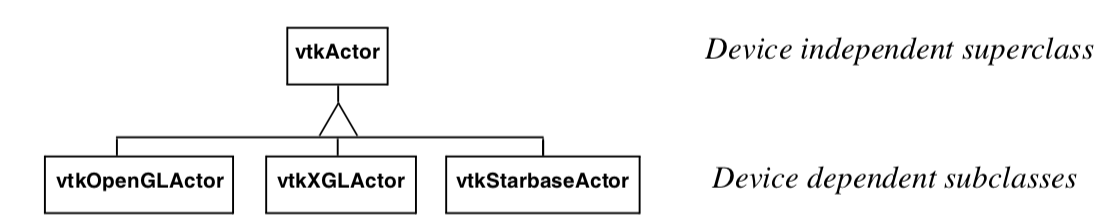
\includegraphics[width=0.96\linewidth]{Figure3-25a}
		\caption{Inheritance of device classes.}
		\label{fig:Figure3-25a}
	\end{subfigure}
	\hfill
	\begin{subfigure}[h]{0.96\linewidth}
		\caption*{}
	\end{subfigure}
	\hfill
	\begin{subfigure}[h]{0.96\linewidth}
		\begin{lstlisting}[language=C++, caption={}]
		vtkActor *vtkActor::New()
		{
		vtkObject* ret = vtkGraphicsFactory::CreateInstance("vtkActor");
		return (vtkActor*)ret;
		}
		\end{lstlisting}
		\caption{Code fragment from vtkActor::New().}
		\label{fig:Figure3-25b}
	\end{subfigure}
	\hfill
	\begin{subfigure}[h]{0.96\linewidth}
		\caption*{}
	\end{subfigure}
	\hfill
	\begin{subfigure}[h]{0.96\linewidth}
		\begin{lstlisting}[language=C++, caption={}]
		if (!strcmp("OpenGL",rl) || !strcmp("Win32OpenGL",rl) ||
		!strcmp("CarbonOpenGL",rl) || !strcmp("CocoaOpenGL",rl))
		{
		if(strcmp(vtkclassname, "vtkActor") == 0)
		{
		return vtkOpenGLActor::New();
		}
		\end{lstlisting}
		\caption{Code fragment from vtkGraphicsFactory::CreateInstance(vtkclassname).}
		\label{fig:Figure3-25cc}
	\end{subfigure}
	\caption{Achieving device independence using (a) inheritance and object factories (b) and (c)..}\label{fig:Figure3-25}
\end{figure}

Figure \ref{fig:Figure3-25} (a) illustrates the use of inheritance to achieve device independence. Certain classes like vtkActor are broken into two parts: a device independent superclass and a device dependent subclass.

\begin{samepage}
The trick here is that the user creates a device dependent
subclass by invoking the special constructor New() in the device independent superclass. For example we would use (in C++)
\begin{lstlisting}[language=C++]
vtkActor *anActor = vtkActor::New()
\end{lstlisting}
\noindent to create a device dependent instance of vtkActor. The user sees no device dependent code, but in actuality anActor is a pointer to a device dependent subclass of vtkActor. Figure \ref{fig:Figure3-25} (b) is a code fragment of the constructor method New() which uses VTK's object factory mechanism. In turn, the vtkGraphicsFactory\index{vtkGraphicsFactory} (used to instantiate graphical classes) produces the appropriate concrete subclass when requested to instantiate an actor as shown in Figure \ref{fig:Figure3-25}.
\end{samepage}

The use of object factories as implemented using the New() method allows us to create device independent code that can move from computer to computer and adapt to changing technology. For example, if a new graphics library became available, we would only have to create a new device dependent subclass, and then modify the graphics factory to instantiate the appropriate sub-class based on environment variables or other system information. This extension would be localized and only done once, and all applications based on these object factories would be automatically ported without change.

This section works through some simple applications implemented with VTK graphics objects. The focus is on the basics: how to create renderers, lights, cameras, and actors. Later chapters tie together these basic principles to create applications for data visualization.

\subsection{Examples}

\begin{description}[leftmargin=0cm,labelindent=0cm]

\item[Render a Cone.] The following C++ code uses most of the objects introduced in this section to create an image of a cone. The vtkConeSource generates a polygonal representation of a cone and vtkPolyDataMapper maps the geometry (in conjunction with the actor) to the underlying graphics library. (The source code to this example can be found in \href{https://lorensen.github.io/VTKExamples/site/Cxx/GeometricObjects/Cone/}{Cone.cxx} or \href{https://lorensen.github.io/VTKExamples/site/Python/GeometricObjects/Cone/}{Cone.py}. The source code contains additional documentation as well.)

\label{eg:render_cone}
\begin{lstlisting}[language=C++, caption={Cone.cxx}, escapechar=\$]
#include "vtkConeSource.h"
#include "vtkPolyDataMapper.h"
#include "vtkRenderWindow.h"
#include "vtkCamera.h"
#include "vtkActor.h"
#include "vtkRenderer.h"

int main( int argc, char *argv[] )
{
  vtkConeSource$\index{vtkConeSource!example}$ *cone = vtkConeSource::New();
    cone->SetHeight( 3.0 );
    cone->SetRadius( 1.0 );
    cone->SetResolution( 10 );

  vtkPolyDataMapper *coneMapper = vtkPolyDataMapper::New();
    coneMapper->SetInputConnection( cone->GetOutputPort() );
  vtkActor *coneActor = vtkActor::New();
    coneActor->SetMapper( coneMapper );

  vtkRenderer *ren1= vtkRenderer::New();
    ren1->AddActor( coneActor );
    ren1->SetBackground( 0.1, 0.2, 0.4 );

  vtkRenderWindow *renWin = vtkRenderWindow::New();
    renWin->AddRenderer( ren1 ); renWin->SetSize( 300, 300 );

  int i;
  for (i = 0; i < 360; ++i)
    {
// render the image
     renWin->Render();
// rotate the active camera by one degree
     ren1->GetActiveCamera()->Azimuth( 1 );
    }
  cone->Delete();
  coneMapper->Delete();
  coneActor->Delete();
// cleanup
  ren1->Delete();
  renWin->Delete();

  return 0;
}\end{lstlisting}

Some comments about this example. The include files vtk*.h include class definitions for the objects in VTK necessary to compile this example. We use the constructor New() to create the objects in this example, and the method Delete() to destroy the objects. In VTK the use of New() and Delete() is mandatory to insure device independence and properly manage reference counting. (See VTK User's Guide for details.) In this example the use of Delete() is really not necessary because the objects are automatically deleted upon program termination. But generally speaking, you should always use a Delete() for every invocation of New(). (Future examples will not show the Delete() methods in the scope of the main() program to conserve space, nor show the required \#include statements.)

The data representing the cone (a set of polygons) in this example is created by linking together a series of objects into a \emph{pipeline}\index{pipeline} (which is the topic of the next chapter). First a polygonal representation of the cone is created with a vtkConeSource and serves as input to the data mapper as specified with the SetInput() method. The SetMapper() method associates the mapper's data with the coneActor. The next line adds coneActor to the renderer's list of actors. The cone is rendered in a loop running over $360^\circ$. Since there are no cameras or lights defined in the above example, VTK automatically generates a default light and camera as a convenience to the user. The camera is accessed through the GetActiveCamera() method, and a one degree azimuth is applied as shown. Each time a change is made to any objects a Render() method is invoked to produce the corresponding image. Once the loop is complete all allocated objects are destroyed and the program exits.

\begin{figure}[!htb]
  \centering
  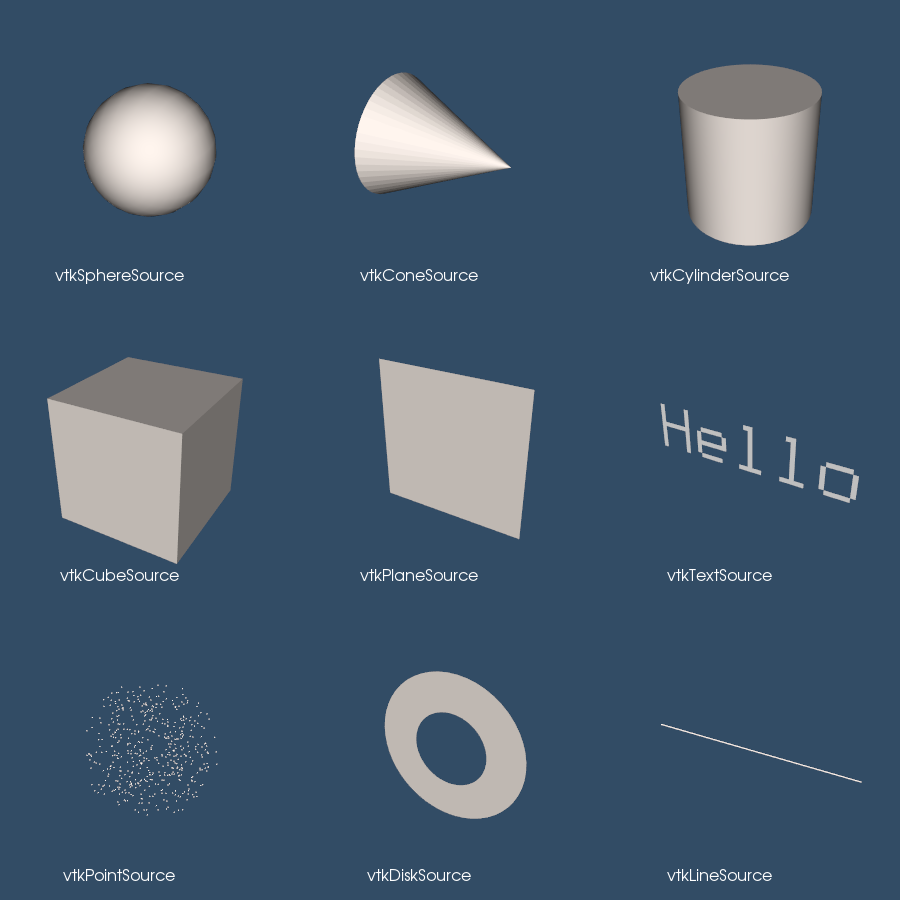
\includegraphics[width=0.8\textwidth]{Figure3-26}\\
  \caption{Examples of source objects that procedurally generate polygonal models. These nine images represent just some of the capability of VTK. From upper left in reading order: sphere, cone, cylinder, cube, plane, text, random point cloud, disk (with or without hole), and line source. Other polygonal source objects are available; check the subclasses of vtkPolyDataAlgorithm. See  \href{https://lorensen.github.io/VTKExamples/site/Cxx/GeometricObjects/SourceObjectsDemo/}{SourceObjectsDemo.cxx} or \href{https://lorensen.github.io/VTKExamples/site/Python/GeometricObjects/SourceObjectsDemo/}{SourceObjectsDemo.py}}\label{fig:Figure3-26}
\end{figure}

There are many different types of source objects in VTK similar to vtkConeSource as shown in Figure \ref{fig:Figure3-26}. In the next chapter we will learn more about source and other types of filters.

\item[Events and Observers.]
\label{sub:examples_events_observers}

A visualization toolkit like VTK is frequently used in interactive applications or may be required to provide status during operation. In addition, integration with other packages such as GUI toolkits is a common task. Supporting such features requires a mechanism for inserting user functionality into the software. In VTK, the \emph{command/observer}\index{command/observer}
 design pattern \cite{Gamma95} is used for this purpose.

Fundamental to this design pattern as implemented in VTK is the concept of \emph{events}\index{events}. An event signals that an important operation has occurred in the software. For example, if the user presses the left mouse button in the render window, VTK will invoke the LeftButtonPressEvent\index{events!LeftButtonPressEvent}. Observers are objects that register their interest in a particular event or events. When one of these events is invoked, the observer\index{observer} receives notification and may perform any valid operation at that point; that is, execute the command associated with the observer. The benefit of the command/observer design pattern is that is simple in concept and implementation, yet provides significant power to the user. However it does require the software implementation to invoke events as it operates.

In the next example, an observer watches for the StartEvent\index{events!StartEvent} invoked by the renderer just as it begins the rendering process. The observer in turn executes its associated command which simply prints out the camera's current position.

\begin{lstlisting}[language=C++, caption={}, escapechar=\$]
#include "vtkCommand.h"
// Callback for the interaction
class vtkMyCallback : public vtkCommand$\index{vtkCommand!example}$
{
public:
  static vtkMyCallback *New()
    { return new vtkMyCallback; }
  virtual void Execute(vtkObject *caller, unsigned long, void*)
    {
      vtkRenderer *ren =
               reinterpret_cast<vtkRenderer*>(caller);
      cout << ren->GetActiveCamera()->GetPosition()[0] << " "
      ren->GetActiveCamera()->GetPosition()[1] << " "
      ren->GetActiveCamera()->GetPosition()[2] << "n";
    }
};

int main( int argc, char *argv[] )
{
  vtkConeSource *cone = vtkConeSource::New();
    cone->SetHeight( 3.0 );
    cone->SetRadius( 1.0 );
    cone->SetResolution( 10 );

  vtkPolyDataMapper *coneMapper = vtkPolyDataMapper::New();
   coneMapper->SetInputConnection(cone->GetOutputPort());
  vtkActor *coneActor = vtkActor::New();
  coneActor->SetMapper( coneMapper );

  vtkRenderer *ren1= vtkRenderer::New();
    ren1->AddActor( coneActor );
    ren1->SetBackground( 0.1, 0.2, 0.4 );

  vtkRenderWindow *renWin = vtkRenderWindow::New();
    renWin->AddRenderer( ren1 ); renWin->SetSize( 300, 300 );

  vtkMyCallback *mo1 = vtkMyCallback::New();
    ren1->AddObserver(vtkCommand::StartEvent,mo1); mo1->Delete();

  int i;
  for (i = 0; i < 360; ++i)
  {
  //   render the image
    renWin->Render();
  // rotate the active camera by one degree
    ren1->GetActiveCamera()->Azimuth( 1 );
  }

  cone->Delete();
  coneMapper->Delete();
  coneActor->Delete();
  ren1->Delete();
  renWin->Delete();
  return 0;
}
\end{lstlisting}

The observer is created by deriving from the class vtkCommand. The Execute() method is required to be implemented by any concrete subclass of vtkCommand (i.e., the method is pure virtual). The resulting subclass, vtkMyCommand, is instantiated and registered with the renderer instance ren1 using the AddObserver() method. In this case the StartEvent\index{StartEvent!example} is the observed event.

This simple example does not demonstrate the true power of the command/observer design pattern. Later in this chapter ( ``Interpreted Code'' on page \pageref{subsec:examples_interpreted_code} ) we will see how this functionality is used to integrate a simple GUI into VTK. In Chapter 7 three--dimensional interaction widgets will be introduced ( ``3D Widgets and User Interaction''  on page \pageref{sec:3D_widgets_user_interaction} ).

\item[Creating Multiple Renderers.]

The next example is a bit more complex and uses multiple renderers that share a single rendering window. We use viewports to define where the renderers should draw in the render window. (This C++ code can be found in Cone3.cxx.)

\begin{figure}[!htb]
  \centering
  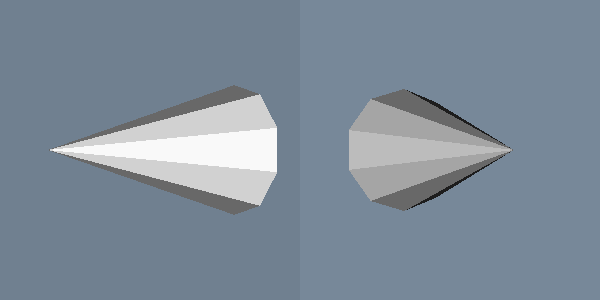
\includegraphics[width=0.8\textwidth]{Figure3-27}\\
  \caption{Two frames of output from Cone3.cxx. See  \href{https://lorensen.github.io/VTKExamples/site/Cxx/Rendering/Cone3/}{Cone3.cxx} or \href{https://lorensen.github.io/VTKExamples/site/Python/Rendering/Cone3/}{Cone3.py}}\label{fig:Figure3-27}
\end{figure}

\begin{lstlisting}[language=C++, caption={Cone3.cxx}]
vtkRenderer *ren1= vtkRenderer::New();
  ren1->AddActor( coneActor );
  ren1->SetBackground( 0.1, 0.2, 0.4 );
  ren1->SetViewport(0.0, 0.0, 0.5, 1.0);

vtkRenderer *ren2= vtkRenderer::New();
  ren2->AddActor( coneActor );
  ren2->SetBackground( 0.2, 0.3, 0.5 );
  ren2->SetViewport(0.5, 0.0, 1.0, 1.0);

vtkRenderWindow *renWin = vtkRenderWindow::New();
  renWin->AddRenderer( ren1 );
  renWin->AddRenderer( ren2 );
  renWin->SetSize( 600, 300 );

ren1->GetActiveCamera()->Azimuth(90);

int i;
for (i = 0; i < 360; ++i)
  {
  // render the image renWin->Render();
  // rotate the active camera by one degree
    ren1->GetActiveCamera()->Azimuth( 1 );
    ren2->GetActiveCamera()->Azimuth( 1 );
  }
\end{lstlisting}

As you can see, much of the code is the same as the previous example. The first difference is that we create two renderers instead of one. We assign the same actor to both renderers, but set each renderer's background to a different color. We set the viewport of the two renderers so that one is on the left half of the rendering window and the other is on the right. The rendering window's size is specified as 600 by 300 pixels, which results in each renderer drawing into a viewport of 300 by 300 pixels.

A good application of multiple renderers is to display different views of the same world as demonstrated in this example. Here we adjust the first renderer's camera with a 90 degree azimuth. We then start a loop that rotates the two cameras around the cone. Figure \ref{fig:Figure3-27} shows two frames from this animation.

\item[Properties and Transformations.]

The previous examples did not explicitly create property or transformation objects or apply actor methods that affect these objects. Instead, we accepted default instance variable values. This procedure is typical of VTK applications. Most instance variables have been preset to generate acceptable results, but methods are always available for you to overide the default values. 

\begin{figure}[!htb]
  \centering
  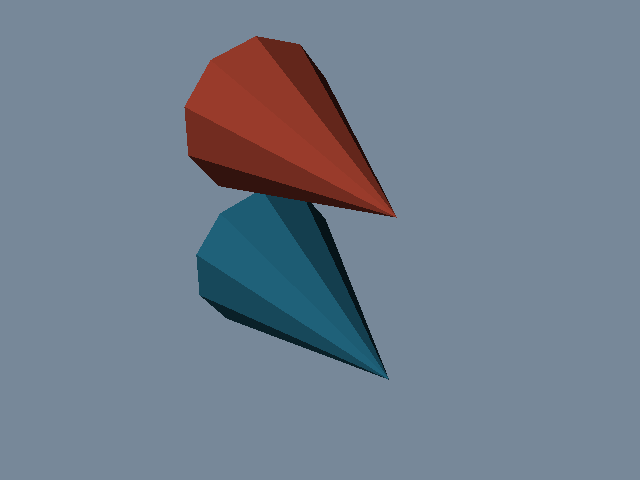
\includegraphics[width=0.8\textwidth]{Figure3-28}\\
  \caption{Modifying properties and transformation matrix. See  \href{https://lorensen.github.io/VTKExamples/site/Cxx/Rendering/Cone4/}{Cone4.cxx} or \href{https://lorensen.github.io/VTKExamples/site/Python/Rendering/Cone4/}{Cone4.py}}\label{fig:Figure3-28}
\end{figure}

This example creates an image of two cones of different colors and specular properties. In addition, we transform one of the objects to lay next to the other. The C++ source code for this example can be found in \href{https://lorensen.github.io/VTKExamples/site/Cxx/Rendering/Cone4/}{Cone4.cxx}.

\begin{lstlisting}[language=C++, caption={Cone4.cxx}]
vtkActor *coneActor = vtkActor::New();
  coneActor->SetMapper(coneMapper);
  coneActor->GetProperty()->SetColor(0.2, 0.63, 0.79);
  coneActor->GetProperty()->SetDiffuse(0.7);
  coneActor->GetProperty()->SetSpecular(0.4);
  coneActor->GetProperty()->SetSpecularPower(20);

vtkProperty *property = vtkProperty::New();
  property->SetColor(1.0, 0.3882, 0.2784);
  property->SetDiffuse(0.7);
  property->SetSpecular(0.4);
  property->SetSpecularPower(20);

vtkActor *coneActor2 = vtkActor::New();
  coneActor2->SetMapper(coneMapper);
  coneActor2->GetProperty()->SetColor(0.2, 0.63, 0.79);
  coneActor2->SetProperty(property);
  coneActor2->SetPosition(0, 2, 0);

vtkRenderer *ren1= vtkRenderer::New();
  ren1->AddActor( coneActor );
  ren1->AddActor( coneActor2 );
  ren1->SetBackground( 0.1, 0.2, 0.4 );
\end{lstlisting}

We set the actor coneActor properties by modifying the property object automatically created by the actor. This differs from actor coneActor2, where we create a property directly and then assign it to the actor. ConeActor2 is moved from its default position by applying the SetPosition() method. This method affects the transformation matrix that is an instance variable of the actor. The resulting image is shown in Figure \ref{fig:Figure3-28}.

\item[Introducing vtkRenderWindowInteractor]
\label{subsec:examples_introducing_vtkRenderWindowInteractor}

The previous examples are not interactive. That is, it is not possible to directly interact with the data without modifying and recompiling the C++ code. One common type of interaction is to change camera position so that we can view our scene from different vantage points. In the \emph{Visualization Toolkit} we have provided a suite of convenient objects to do this: vtkRenderWindowInteractor\index{vtkRenderWindowInteractor}, vtkInteractorStyle\index{vtkInteractorStyle} and their derived classes.

Instances of the class vtkRenderWindowInteractor capture windowing system specific mouse and keyboard events in the rendering window, and then translate these events into VTK events. For example, mouse motion in an X11 or Windows application (occurring in a render window) would be translated by vtkRenderWindowInteractor into VTK's MouseMoveEvent\index{events!MouseMoveEvent}. Any observers\index{events!See also observers} registered for this event would be notified (see ``Events and Observers'' on \pageref{sub:examples_events_observers} ). Typically an instance of vtkInteractorStyle is used in combination with vtkRenderWindowInteractor to define a behavior associated with particular events. For example, we can perform camera dolly, pan, and rotation by using different mouse button and motion combinations. The following code fragment shows how to instantiate and use these objects. This example is the same as our first example with the addition of the interactor and interactor style. The complete example C++ code is in Cone5.cxx.

\begin{lstlisting}[language=C++, caption={Cone5.cxx}, escapechar=\$]
vtkRenderWindowInteractor *iren =
  vtkRenderWindowInteractor::New();

  iren->SetRenderWindow(renWin);

vtkInteractorStyleTrackballCamera$\index{vtkInteractorStyleTrackballCamera!example}$ *style =
 vtkInteractorStyleTrackballCamera::New();

  iren->SetInteractorStyle(style);
  iren->Initialize();
  iren->Start();
\end{lstlisting}

After the interactor is created using its New() method, we must tell it what render window to capture events in using the SetRenderWindow() method. In order to use the interactor we have to initialize and start the event loop using the Initialize() and Start() methods, which works with the event loop of the windowing system to begin to catch events. Some of the more useful events include the ``w'' key, which draws all actors in wireframe; the ``s'' key, which draws the actors in surface form; the ``3'' key, which toggles in and out of 3D stereo for those systems that support this; the ``r'' key, which resets camera view; and the " e" key, which exits the application. In addition, the mouse buttons rotate, pan, and dolly about the camera's focal point. Two advanced features are the ``u'' key, which executes a user-defined function; and the ``p'' key, which picks the actor under the mouse pointer.

\item[Interpreted Code.]
\label{subsec:examples_interpreted_code}

In the previous example we saw how to create an interactor style object in conjunction with vtkRenderWindowInteractor to enable us to manipulate the camera by mousing in the render window. Although this provides flexibility and interactivity for a large number of applications, there are examples throughout this text where we want to modify other parameters. These parameters range from actor properties, such as color, to the name of an input file. Of course we can always write or modify C++ code to do this, but in many cases the turn-around time between making the change and seeing the result is too long. One way to improve the overall interactivity of the system is to use an interpreted interface. Interpreted systems allow us to modify objects and immediately see the result, without the need to recompile and relink source code. Interpreted languages also provide many tools, such as GUI (Graphical User Interface) tools, that simplify the creation of applications.

\begin{minipage}{.6\linewidth}
The \emph{Visualization Toolkit} has built into its compilation process the ability to automatically generate language bindings to the interpreted languages Tcl\index{interpreted languages!Tcl}\index{Tcl}, Python\index{interpreted languages!Python}\index{Python} and Java\index{interpreted languages!Java}\index{Java} [Ousterhout94]. This so-called wrapping process automatically creates a layer between the C++ VTK library and the interpreter as illustrated in Figure \ref{fig:Figure3-29}. There is a one-to-one mapping between C++ methods and Tcl C++ functions for most objects and methods in the system. To demonstrate this, the following example repeats the previous C++ example except that it is implemented with a Tcl script. (The script can be found in Cone5.tcl).
\end{minipage}
\hfill
\begin{minipage}{.25\linewidth}
  \centering
  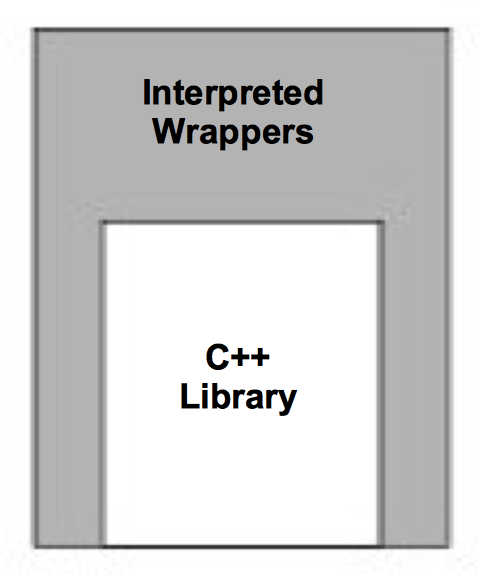
\includegraphics[width=0.6\linewidth]{Figure3-29} 
  \captionof{figure}{In VTK the C++ library is automatically wrapped with the interpreted languages Tcl, Python, and Java.}
  \label{fig:Figure3-29}
\end{minipage}

\begin{lstlisting}[language=TCL, caption={Cone5.tcl}, escapechar=\% ]
package require vtk%\index{package require!vtk}%
package require%\index{Tcl!package require}% vtkinteraction%\index{package require!vtkinteraction}%
vtkConeSource cone
  cone SetHeight 3.0
  cone SetRadius 1.0
  cone SetResolution 10

vtkPolyDataMapper coneMapper
  coneMapper SetInputConnection [cone GetOutputPort]

vtkActor coneActor
  coneActor SetMapper coneMapper

vtkRenderer ren1
  ren1 AddActor coneActor
  ren1 SetBackground 0.1 0.2 0.4

vtkRenderWindow renWin
  renWin AddRenderer ren1
  renWin SetSize 300 300

vtkRenderWindowInteractor iren
  iren SetRenderWindow renWin

vtkInteractorStyleTrackballCamera style
  iren SetInteractorStyle style
  iren AddObserver#\index{Tcl!AddObserver}# UserEvent {wm deiconify .vtkInteract}
  iren Initialize

wm withdraw .
\end{lstlisting}

\begin{figure}[!htb]
  \centering
  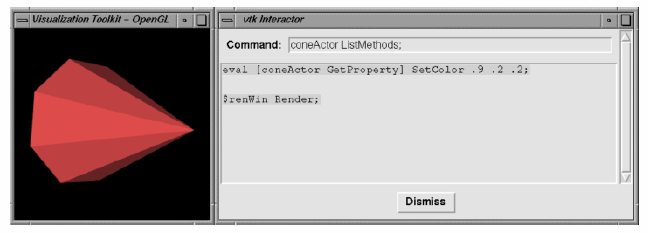
\includegraphics[width=0.8\textwidth]{Figure3-30}\\
  \caption{Using Tcl and Tk to build an interpreted application (Cone5.tcl).}\label{fig:Figure3-30}
\end{figure}

The example begins by loading some shared libraries defining various VTK classes. Next the standard visualization pipeline is created from the vtkConeSource and vtkPolyDataMapper. The rendering classes are created exactly the same as with the C++ example. One major addition is an observer to watch for a UserEvent in the rendering window (by default a ``keypress-u''). The observer triggers the invocation of a Tcl script to raise a Tk interactor GUI widget called vtkInteract. This GUI, which allows the direct typing of Tcl statements, is shown in Figure \ref{fig:Figure3-30} and is defined by the Tcl command package require vtkinteraction which was executed earlier in the script. (Note: Tk is a popular GUI toolkit for interpreted languages and is distributed as part of Tcl.) 

As we can see from this example, the number of lines of code is less for the Tcl example than for equivalent C++ code. Also, many of the complexities of C++ are hidden using the interpreted language. Using this user-interface GUI we can create, modify, and delete objects, and modify their instance variables. The resulting changes appear as soon as a Render() method is applied or mouse events in the rendering window cause a render to occur. We encourage you to use Tcl (or one of the other interpreters) for rapid creation of graphics and visualization examples. C++ is best used when you desire higher performing applications.

\end{description}

\subsubsection{Transformation Matrices}
\label{subsubsec:transform_matrices}
\index{transformation matrix!implementation|(}

Transformation matrices are used throughout the  Visualization Toolkit. Actors (subclasses of vtkProp3D --- see ``Assemblies and Other Types of vtkProp'' on page \pageref{subsubsec:assemblies_vtkprop} ) use them to position and orient\index{orientation} themselves. Various filters, including vtkGlyph3D\index{vtkGlyph3D} and vtkTransformFilter, use transformation matrices to implement their own functionality. As a user you may never use transformation matrices directly, but understanding them is important to successful use of many VTK classes.

The most important aspect to applying transformation matrices\index{transformation matrix!order of application} is to understand the order in which the transformations are applied. If you break down a complex series of transformations into simple combinations of translation, scaling, and rotation, and keep careful track of the order of application, you will have gone a long way to mastering their use.

A good demonstration example of transformation matrices is to examine how vtkActor\index{vtkActor} uses its internal matrix. vtkActor has an internal instance variable Transform to which it delegates many of its methods or uses the matrix to implement its methods. For example, the RotateX(), RotateY(),and RotateZ() methods are all delegated to Transform. The method SetOrientation() uses Transform to orient the actor. The vtkActor class applies transformations in an order that we feel is natural to most users.

The vtkActor class applies transformations in an order that we feel is natural to most users. As a convenience, we have created instance variables that abstract the transformation matrices. The Origin\index{actor!origin}\index{origin!actor} $(o_x,o_y,o_z)$ specifies the point that is the center of rotation and scaling. The Position\index{actor!position}\index{position!actor} $(p_x, p_y, p_z)$p specifies a final translation of the object. Orientation\index{actor!orientation}\index{orientation!actor} $(r_x, r_y, r_z)$ defines the rotation\index{actor!rotation}\index{rotation!and actor} about the $x, y$ and $z$ axes. Scale\index{actor!scale} $(s_x, s_y, s_z)$ defines scale factors for the $x, y,$ and $z$ axes. Internally, the actor uses these instance variables to create the following sequence of transformations (see Equation \eqref{eq:3.6}, Equation \eqref{eq:3.9},  Equation \eqref{eq:3.13}.

\begin{equation}\label{eq:3.14}
T = T_T(p_x + o_{x'}p_y + o_{y'}p_y + o_z)T_{R_z}T_{R_x}T_{R_z}T_ST_T(-o_x,-o_y,-o_z)
\end{equation}
\myequations{vtkActor transforms}

The term $T_T(x, y, z)$ denotes the translations in the $x,y$ and $z$ direction. Recall that we premultiply the transformation matrix times the position vector. This means the transformations are read from right to left. In other words, Equation \eqref{eq:3.14} proceeds as follows:

\begin{enumerate}
\item Translate the actor to its origin. Scaling and rotation will occur about this point. The initial translation will be countered by a translation in the opposite direction after scaling and rotations are applied.

\item Scale the geometry.

\item Rotate the actor about the emph{y}, then emph{x}, and then emph{z} axes.

\item Undo the translation of step 1 and move the actor to its final location.
\end{enumerate}

The order of the transformations is important. In VTK the rotations are ordered to what is natural in most cases. We recommend that you spend some time with the software to learn how these transformations work with your own data.

Probably the most confusing aspect of transformations are rotations and their effect on the Orientation instance variable. Generally orientations are not set directly by the user, and most users will prefer to specify rotations with the RotateX(), RotateY(), and RotateZ() methods. These methods perform rotations about the $x$, $y$, and $z$ axes in an order specified by the user. New rotations are applied to the right of the rotation transformation. If you need to rotate your actor about a single axis, the actor will rotate exactly as you expect it will, and the resulting orientation vector will be as expected. For example, the operation RotateY(20) will produce an orientation of $(0,20,0)$ and a RotateZ(20) will produce $(0,0,20)$. However, a RotateY(20) followed by a RotateZ(20) will not produce $(0,20,20)$ but produce an orientation of $(6.71771, 18.8817, 18.8817)$! This is because the rotation portion of Equation \eqref{eq:3.14} is built from the rotation order emph{z}, then emph{x}, and then emph{y}. To verify this, a RotateZ(20) followed by a RotateY(20) does produce an orientation of $(0,20,20)$. Adding a third rotation can be even more confusing.

A good rule of thumb is to only use the SetOrientation() method to either reset the orientation to $(0,0,0)$ or to set just one of the rotations. The RotateX(), RotateY(), and RotateZ() methods are preferred to SetOrientation() when multiple angles are needed. Remember that these rotations are applied in reverse order. Figure \ref{fig:Figure3-31} illustrates the use of the rotation methods. We turn off the erase between frames using the render window's EraseOff() method so we can see the effects of the rotations. Note that in the fourth image the cow still rotates about her own y axis even though an emph{x} axis rotation preceded the emph{y} rotation.

\begin{figure}[!htb]
  \centering
  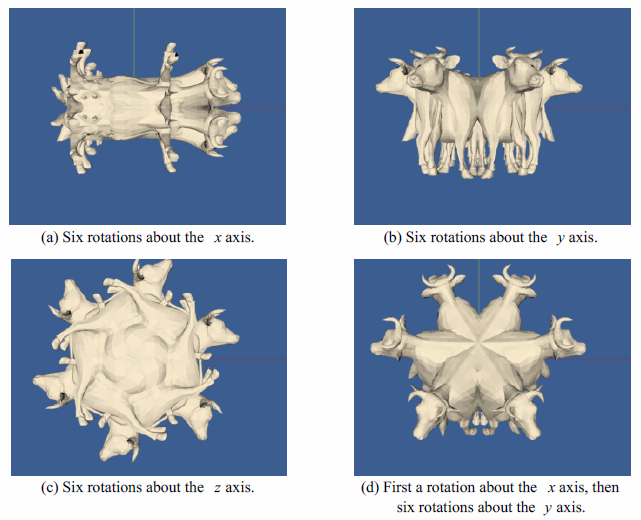
\includegraphics[width=0.8\textwidth]{Figure3-31}\\
  \caption{Rotations of a cow about her axes. In this model, the emph{x} axis is from the left to right; the emph{y} axis is from bottom to top; and the emph{z} axis emerges from the image. The camera location is the same in all four images.}\label{fig:Figure3-31}
\end{figure}


We have seen that VTK hides some of the complexities of matrix transformations by using instance variables that are more natural than a transformation matrix. But there will be times when the predefined order of transformations performed by the actor will not be sufficient. vtkActor has an instance variable UserMatrix that contains a 4 x 4 transformation matrix. This matrix is applied before the transformation composed by the actor. As you become more comfortable with 4 x 4 transformation matrices you may want to build your own matrix. The object vtkTransform creates and manipulates these matrices. Unlike an actor, an instance of vtkTransform does not have an instance variable for position, scale, origin, etc. You control the composition of the matrix directly.

The following statements create an identical 4 x 4 matrix that the actor creates:

\begin{lstlisting}[language=TCL, caption={}]
vtkTransform *myTrans = vtkTransform::New ();
  myTrans->Translate(position[0],position[1],position[2]);
  myTrans->Translate(origin[0],origin[1],origin[2]);
  myTrans->RotateZ(orientation[2]);
  myTrans->RotateX (orientation[0]);
  myTrans->RotateZ(orientation[1];
  myTrans->Scale (scale[0],scale[1],scale[2]);
  myTrans->Translate (-origin[0],-origin[1],-origin[2]);
\end{lstlisting}

Compare this sequence of transform operations with the transformation in Equation \eqref{eq:3.14}.

Our final example shows how the transform built with vtkTransform compares with a transform built by vtkActor. In this example, we will transform our cow so that she rotates about the world coordinate origin $(0,0,0)$. She will appear to be walking around the origin. We accomplish this in two ways: one using vtkTransform and the actor's UserMatrix, then using the actor's instance variables.

First, we will move the cow five feet along the $z$ axis then rotate her about the origin. We always specify transformations in the reverse order of their application:

\begin{lstlisting}[language=C++, caption={}]
vtkTransform *walk = vtkTransform::New(); walk->RotateY(0,20,0);
  walk->Translate(0,0,5);

vtkActor *cow=vtkActor::New();
  cow->SetUserMatrix(walk->GetMatrix());
\end{lstlisting}

These operations produce the transformation sequence:

\begin{equation}\label{eq:3.15}
T=T_T(0,0,5-(-5))T_{R_y}T_ST_T(0,0,-(-5))
\end{equation}

Now we do the same using the cow's instance variables:

\begin{lstlisting}[language=C++, caption={}]
vtkActor *cow=vtkActor::New();
  cow->SetOrigin(0,0,-5);
  cow->RotateY(20);
  cow->SetPosition(0,0,5);
\end{lstlisting}

These operations produce the transformation sequence:

\begin{equation}\label{eq:3.16}
T=T_T(0,0,5-(-5))T_{R_y}T_ST_T(0,0,-(-5))
\end{equation}

Cancelling the minus signs in the right-most translation matrix and combining the position and origin translation produce the equivalent transform that we built with vtkTransform. Figure \ref{fig:Figure3-31} shows the cow rotating with the specified transformation order. Your preference is a matter of taste and how comfortable you are with matrix transformations. As you become more skilled (and your demands are greater) you may prefer to always build your transformations. VTK gives you the choice.

There is one final and powerful operation that affects an actor's orientation. You can rotate an actor about an arbitrary vectoremph\index{rotation!about a vector} positioned at the actor's origin. This is done with the actor's (and transform's) RotateWXYZ() method. The first argument of the operation specifies the number of degrees to rotate about the vector specified by the next three arguments. Figure \ref{fig:Figure3-32} shows how to rotate the cow about a vector passing through her nose. At first, we leave the origin at $(0,0,0)$. This is obviously not what we wanted. The second figure shows the rotation when we change the cow's rotation origin to the tip of her nose.

\begin{figure}[!htb]
  \centering
  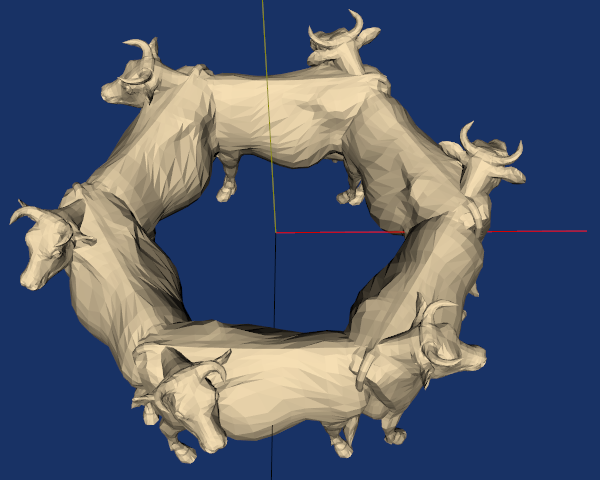
\includegraphics[width=0.8\textwidth]{Figure3-32}\\
  \caption{Modifying properties and transformation matrix. See \href{https://lorensen.github.io/VTKExamples/site/Cxx/Rendering/WalkCow/}{WalkCow.cxx} or \href{https://lorensen.github.io/VTKExamples/site/Python/Rendering/WalkCow/}{WalkCow.py}}\label{fig:Figure3-32}
\end{figure}

\begin{figure}
\begin{subfigure}[h]{0.48\linewidth}
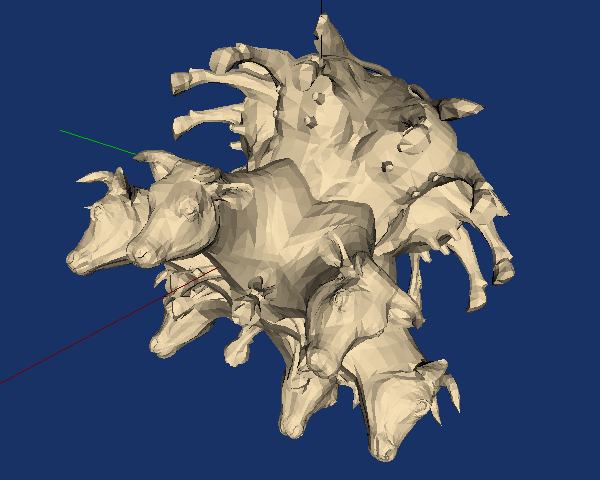
\includegraphics[width=\linewidth]{Figure3-33a}
\caption{With origin $(0,0,0)$.(\href{https://lorensen.github.io/VTKExamples/site/Cxx/Rendering/WalkCowA/}{WalkCowA.cxx} or \href{https://lorensen.github.io/VTKExamples/site/Python/Rendering/WalkCowA/}{WalkCowA.py})}
\end{subfigure}
\hfill
\begin{subfigure}[h]{0.48\linewidth}
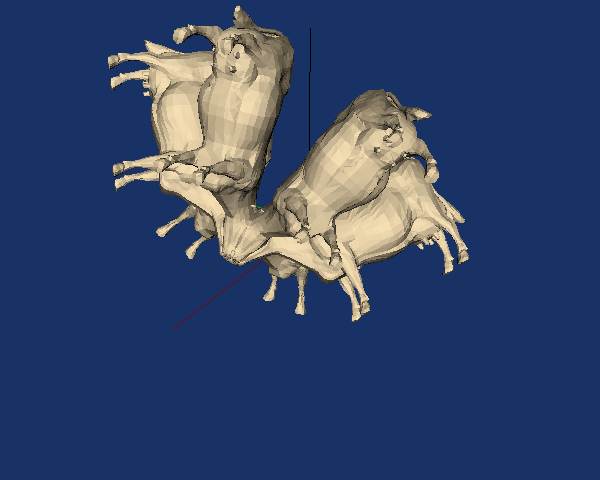
\includegraphics[width=\linewidth]{Figure3-33b}
\caption{With origin at $(6.1,1.3,.02)$.(\href{https://lorensen.github.io/VTKExamples/site/Cxx/Rendering/WalkCowB/}{WalkCowB.cxx} or \href{https://lorensen.github.io/VTKExamples/site/Python/Rendering/WalkCowB/}{WalkCowB.py})}
\end{subfigure}%
\caption{The cow rotating about a vector passing through her nose.}
\end{figure}
\index{transformation matrix!implementation|)}

\subsubsection{Assemblies and Other Types of vtkProp}
\label{subsubsec:assemblies_vtkprop}
\index{assembly}

Often it is desirable to collect actors into a hierarchy of transform-dependent groups. For example, a robot arm may be represented by rigid links connected at joints such as the shoulder joint, upper arm, elbow, lower arm, wrist joint, and hand. In such a configuration, when the shoulder joint rotates, the expected behavior is that the entire arm rotates since the links are connected together. This is an example of what is referred to as an \emph{assembly} in VTK\index{assembly!parts}. vtkAssembly\index{vtkAssembly} is just one of many actor--like classes in VTK. As Figure \ref{fig:Figure3-34} shows, these classes are arranged into a hierarchy of vtkProps. (In stage and film terminology, a prop is something that appears or is used on stage.) Assemblies are formed in VTK by instantiating a vtkAssembly and then adding \emph{parts} to it. A part is any instance of vtkProp3D ---including other assemblies. This means that assemblies can be formed into hierarchies (as long as they do not contain self-referencing loops). Assemblies obey the rules of transformation concatenation illustrated in the previous section (see ``Transformation Matrices'' on page \pageref{subsubsec:transform_matrices} ). Here is an example of how to create a simple assembly hierarchy (from assembly.tcl ).

\index{assembly!example}
\begin{lstlisting}[language=TCL, caption={Part of assembly.tcl}, escapechar=\%]
vtkSphereSource sphere
vtkPolyDataMapper sphereMapper
  sphereMapper SetInputConnection [sphere GetOutputPort] vtkActor
sphereActor
  sphereActor SetMapper sphereMapper
  sphereActor SetOrigin 2 1 3
  sphereActor RotateY 6
  sphereActor SetPosition 2.25 0 0
  [sphereActor GetProperty] SetColor 1 0 1

vtkCubeSource cube
vtkPolyDataMapper cubeMapper
  cubeMapper SetInputConnection [cube GetOutputPort] vtkActor
cubeActor
  cubeActor SetMapper cubeMapper
  cubeActor SetPosition 0.0 .25 0
  [cubeActor GetProperty] SetColor 0 0 1
vtkConeSource cone
vtkPolyDataMapper coneMapper
  coneMapper SetInputConnection [cone GetOutputPort] vtkActor
coneActor
  coneActor SetMapper coneMapper
  coneActor SetPosition 0 0 .25
  [coneActor GetProperty] SetColor 0 1 0
vtkCylinderSource cylinder
vtkPolyDataMapper cylinderMapper
  cylinderMapper SetInputConnection [cylinder GetOutputPort]
  cylinderMapper SetResolveCoincidentTopologyToPolygonOffset

vtkActor cylinderActor
  cylinderActor SetMapper cylinderMapper
  [cylinderActor GetProperty] SetColor 1 0 0

vtkAssembly%\index{vtkAssembly!example}% assembly
  assembly AddPart cylinderActor
  assembly AddPart sphereActor
  assembly AddPart cubeActor
  assembly AddPart coneActor
  assembly SetOrigin 5 10 15

// allows faces a specified camera and is used for billboards.
  assembly AddPosition 5 0 0
  assembly RotateX 15
  ren1 AddActor assembly
  ren1 AddActor coneActor
}
\end{lstlisting}

\begin{figure}[!htb]
\floatbox[{\capbeside\thisfloatsetup{capbesideposition={left,center},capbesidewidth=0.4\textwidth}}]{figure}[\FBwidth]
{\caption{The vtkProp hierarchy.
Props that can be transformed in 3D space are a subclass of
vtkProp3D. Images can be drawn effectively with vtkImageActor.
Overlay text and graphics use vtkActor2D\index{vtkActor2D}. Hierarchical groups
of vtkProps are gathered into a vtkPropAssembly. Volume rendering
uses vtkVolume. Collections of transformable props create a
vtkAssembly\index{vtkAssembly}. Level--of--detail rendering uses vtkLODProp3D\index{vtkLODProp3D} and
vtkLODActor\index{vtkLODActor}. A vtkFollower\index{vtkFollower} faces a specified camera
and is used for billboards.}\label{fig:Figure3-34}}
{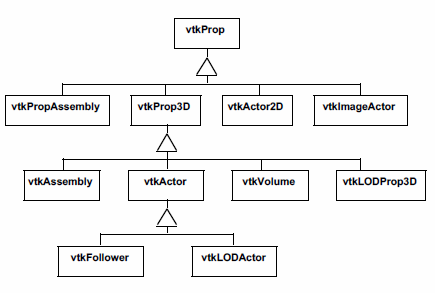
\includegraphics[width=0.6\textwidth]{Figure3-34}}
\end{figure}

Note that in this example various actors are added to the assembly with the AddPart() method. The top-level element of the assembly is the only prop in the hierarchy added to the renderer (with AddActor()). Note also that the coneActor appears twice: once as a part of the assembly, and once as a separate actor added to the renderer with AddActor(). As you might imagine, this means that the rendering of assemblies requires concatenation of transformation matrices to insure the correct positioning of each vtkProp3D. Furthermore, hierarchical assemblies require special treatment during picking (i.e., graphically selecting props) since a vtkProp can appear more than once in different assembly hierarchies. Picking issues are discussed in more detail in ``Picking'' on page \pageref{subsec:picking}.

As Figure \ref{fig:Figure3-34} indicates, there are other types of vtkProp as well. Most of these will be informally described in the many examples found in this book. In particular, extensive coverage is given to vtkVolume when we describe volume rendering (see ``Volume Rendering'' on page \pageref{sec:volume_rendering}).


\section{Chapter Summary}

Rendering is the process of generating an image using a computer. Computer graphics is the field of study that encompasses rendering techniques, and forms the foundation of data visualization.

Three--dimensional rendering techniques simulate the interaction of lights and cameras with objects, or actors, to generate images. A scene consists of a combination of lights, cameras, and actors. Object-order rendering techniques generate images by rendering actors in a scene in order. Image-order techniques render the image one pixel at a time. Polygon based graphics hardware is based on object-order techniques. Ray tracing or ray-casting is an image-order technique.

Lighting models require a specification of color. We saw both the RGB (red-green-blue) and HSV (hue-saturation-value) color models. The HSV model is a more natural model than the RGB model for most users. Lighting models also include effects due to ambient, diffuse, and specular lighting.

There are four important coordinate systems in computer graphics. The model system is the 3D coordinate system where our geometry is defined. The world system is the global Cartesian system. All modelled data is eventually transformed into the world system. The view coordinate system represents what is visible to the camera. It is a 2D system scaled from $(-1,1)$. The display coordinate system uses actual pixel locations on the computer display.

Homogeneous coordinates are a 4D coordinate system in which we can include the effects of perspective transformation. Transformation matrices are \(4 \times 4\) matrices that operate on homogeneous coordinates. Transformation matrices can represent the effects of translation, scaling, and rotation of an actor. These matrices can be multiplied together to give combined transformations.

Graphics programming is usually implemented using higher-level graphics libraries and specialized hardware systems. These dedicated systems offer better performance and easier implementation of graphics applications. Common techniques implemented in these systems include dithering and z-buffering. Dithering is a technique to simulate colors by mixing combinations of available colors. Z-buffering is a technique to perform hidden-line and hidden-surface removal.

\section{Bibliographic Notes}
\label{Ch03BibNotes}

This chapter provides the reader with enough information to understand the basic issues and terms used in computer graphics. There are a number of good text books that cover computer graphics in more detail and are recommended to readers who would like a more thorough understanding. The bible of computer graphics is \cite{FoleyVanDam90}. For those wishing for less intimidating books \cite{BurgerGillies89} and \cite{Watt93} are also useful references. You also may wish to peruse proceedings of the ACM SIGGRAPH conferences. These include papers and references to other papers for some of the most important work in computer graphics. \cite{Carlson85} provides a good introduction for those who wish to learn more about the human vision system.


\printbibliography


\section{Exercises}
\begin{enumerate}

\item Estimate the odds of a ray of light being emitted from the sun, traveling to earth and hitting a one meter square picnic blanket. You can assume that the sun is a point light source that emits light uniformly in all directions. 
The approximate distance from the sun to the earth is 150,000,000km.

\begin{enumerate}

    \item What are the odds when the sun is directly overhead?

    \item What are the odds when the sun is inclined 45 degrees relative to the surface normal of the picnic blanket?

    \item What assumptions or approximations did you make?

\end{enumerate}

\item Proceeding from your result of Exercise 3.1, what are the difficulties in determining the odds of a ray of light traveling from the sun to hit the picnic blanket and then entering a viewer's eye?

\item The color cyan can be represented in both the HSV and RGB color spaces as shown in Table \ref{table:Figure3-4}. These two representations for cyan do not yield the same wavelength intensity plots. How do they differ?

\item The vtkSphereSource class generates a polygonal model of a sphere.
Using the examples at the end of this chapter as starting points, create a program to display a white sphere.
Set the ambient and diffuse intensities to 0.5. Then add a for-loop to this program that adjusts the ambient and diffuse color of this sphere so that as the loop progresses, the diffuse color goes from red to blue, and the ambient color goes from blue to green.
You might also try adjusting other lighting parameters such as specular color, ambient, diffuse, and specular intensity.

\item Using the vtkSphereSource as described in Exercise 3.4, create a program to display the sphere with a light source positioned at $(1,1,1)$. Then extend this program by adding a for loop that will adjust the active camera's clipping range so that increasing portions of the interior of the sphere can be seen.
By increasing the first value of the clipping range, you will be adjusting the position of the front clipping plane.
Once the front clipping plane starts intersecting the sphere, you should be able to see inside of it.
The default radius of the vtkSphereSource is 0.5, so make sure that you adjust the clipping range in increments less than 1.0.

\item Modify the program presented in ``Render a Cone'' on page \pageref{eg:render_cone} so that the user can enter in a world coordinate in homogenous coordinates and the program will print out the resulting display coordinate. Refer to the reference page for vtkRenderer for some useful methods.

\begin{enumerate}

    \item Are there any world coordinates that you would expect to be undefined in display coordinates?

    \item What happens when the world coordinates are behind the camera?

\end{enumerate}

\item Consider rasterizing a ten by ten pixel square. Contrast the approximate difference in the number of arithmetic operations that would need to be done for the cases where it is flat, Gouraud, or Phong shaded.

\item When using a z-buffer, we must also interpolate the z-values (or depth) when rasterizing a primitive. Working from Exercise 3.7, what is the additional burden of computing z-buffer values while rasterizing our square?

\item vtkTransform has a method GetOrientation() that looks at the resulting transformation matrix built from a series of rotations and provides the single x, y, and z rotations that will reproduce the matrix. Specify a series of rotations in a variety of orders and request the orientation with GetOrientation(). Then apply the rotations in the same order that vtkActor does and verify that the resulting 4 x 4 transformation matrix is the same.

\item vtkTransform, by default, applies new transformations at the right of the current transformation. The method PostMultiply() changes the behavior so that the transformations are applied to the left.

\begin{enumerate}

\item Use vtkTransform to create a transform using a variety of transformation operators including Scale(), RotateXYZ(), and Translate(). Then create the same matrix with PostMultiplyOn().

\item Applying rotations at the right of a series of transformations in effect rotates the object about its own coordinate system. Use the rotations.tcl script to verify this. Can you explain this?

\item Applying rotations at the left of a series of transformations in effect rotates the object about the world coordinate system. Modify the rotations.tcl script to illustrate this. (Hint: you will have to create an explicit transform with vtkTransform and set the actor's transform with SetUserMatrix().)

\end{enumerate}

\end{enumerate}
